%%%%%%%%%%%%%%%%%%%%%%%%%%%%%%%%%%%%%%%%%%%%%%%%%%%%%%%%%%%%
% PAPER ACADÉMICO - INDICADOR DE VULNERABILIDAD EXTERNA
% A Model-Implied External Vulnerability Indicator for Emerging Markets
%%%%%%%%%%%%%%%%%%%%%%%%%%%%%%%%%%%%%%%%%%%%%%%%%%%%%%%%%%%%

\documentclass[12pt,a4paper]{article}

% --- CODIFICACIÓN & IDIOMA ---
\usepackage[utf8]{inputenc}
\usepackage[T1]{fontenc}
\usepackage[english]{babel}

% --- TIPOGRAFÍA & MICROTIPOGRAFÍA ---
\usepackage{lmodern}
\usepackage[protrusion=true,expansion=true]{microtype}

% --- MATEMÁTICAS ---
\usepackage{amsmath, amssymb, amsthm}
\usepackage{mathtools}
\numberwithin{equation}{section}

% --- TEOREMAS Y DEFINICIONES ---
\newtheorem{proposition}{Proposition}[section]
\newtheorem{lemma}[proposition]{Lemma}
\newtheorem{theorem}[proposition]{Theorem}
\newtheorem{corollary}[proposition]{Corollary}
\theoremstyle{definition}
\newtheorem{definition}[proposition]{Definition}
\newtheorem{assumption}[proposition]{Assumption}
\theoremstyle{remark}
\newtheorem{remark}[proposition]{Remark}
\newtheorem{example}[proposition]{Example}

% --- TABLAS PROFESIONALES ---
\usepackage{booktabs}
\usepackage{threeparttable}
\usepackage{multirow}
\usepackage{siunitx}
\sisetup{
  output-decimal-marker = {.},
  table-number-alignment = center,
  table-figures-integer = 3,
  table-figures-decimal = 3
}

% --- FIGURAS & GRÁFICOS ---
\usepackage{graphicx}
\graphicspath{{../../notebooks/figures/}}
\usepackage[font=small,labelfont=bf,labelsep=period]{caption}
\usepackage{subcaption}
\usepackage{placeins}

% --- COLOR ---
\usepackage{xcolor}
\definecolor{brandblue}{HTML}{0D3B66}
\definecolor{brandorange}{HTML}{F4A261}

% --- LISTAS ---
\usepackage{enumitem}
\setlist{nosep,leftmargin=*}

% --- HIPERVÍNCULOS & REFERENCIAS ---
\usepackage{hyperref}
\hypersetup{
  colorlinks=true,
  linkcolor=brandblue,
  citecolor=brandblue,
  urlcolor=brandblue,
  pdfauthor={Manuel Alejandro Hidalgo Pérez, Ernesto Talvi},
  pdftitle={A Model-Implied External Vulnerability Indicator for Emerging Markets}
}
\usepackage[nameinlink,capitalise,noabbrev]{cleveref}

% --- CITADO ---
\usepackage{csquotes}
\usepackage[style=apa,backend=biber]{biblatex}
\DeclareLanguageMapping{english}{english-apa}
\addbibresource{references.bib}

% --- MÁRGENES ---
\usepackage[left=2.5cm, right=2.5cm, top=3cm, bottom=3cm]{geometry}
\usepackage{parskip}

% --- COMANDOS ÚTILES ---
\newcommand{\vect}[1]{\boldsymbol{#1}}
\DeclareMathOperator{\Var}{Var}
\DeclareMathOperator{\Cov}{Cov}
\DeclareMathOperator{\E}{\mathbb{E}}
\newcommand{\R}{\mathbb{R}}

% --- TÍTULO ---
\title{
  \Large{\textbf{A Model-Implied External Vulnerability Indicator\\
  for Emerging Markets:\\
  Theory, Construction, and Empirical Validation}}\\[1em]
  \normalsize{An Application to Brazil (2000--2024)}
}

\author{
  Manuel Alejandro Hidalgo Pérez\thanks{Universidad Pablo de Olavide and Real Instituto Elcano. Email: \texttt{mahidper@upo.es}} 
  \and 
  Ernesto Talvi\thanks{Real Instituto Elcano. Email: \texttt{etalvi@rielcano.org}}
}

\date{\today}

\begin{document}
\maketitle
\thispagestyle{empty}

\begin{abstract}
\noindent
We develop a model-implied external vulnerability indicator for commodity-exporting emerging markets that integrates three dimensions: long-run disequilibrium (from VECM error correction terms), sensitivity to external shocks (from impulse response functions), and time-varying external risk (from rolling shock covariances). Unlike ad-hoc composite indices, all weights derive endogenously from estimated parameters, ensuring objectivity, traceability, and temporal comparability. Applied to Brazil (2000--2024), the indicator successfully identifies known stress episodes and exhibits significant predictive power for GDP growth at 1--2 quarter horizons (correlation $-0.22$, excluding COVID-19). Full decomposability enables attribution to specific channels (trade vs. financial), making it actionable for policy. The framework is portable across countries with minimal calibration, requiring only three hyperparameters: forecast horizon, covariance window, and risk amplifier intensity.
\end{abstract}

\vspace{0.5cm}

\noindent\textbf{Keywords:} External vulnerability, VECM, early warning systems, emerging markets, Brazil, cointegration, impulse responses

\noindent\textbf{JEL Classification:} F32, F41, C32, E44, O54

\clearpage
\tableofcontents
\clearpage


%%%%%%%%%%%%%%%%%%%%%%%%%%%%%%%%%%%%%%%%%%%%%%%%%%%%%%%%%%%%
% 1. INTRODUCTION
%%%%%%%%%%%%%%%%%%%%%%%%%%%%%%%%%%%%%%%%%%%%%%%%%%%%%%%%%%%%

\section{Introduction}

\subsection{The Challenge of External Vulnerability in Commodity Exporters}

Emerging market economies that rely heavily on commodity exports face structural exposure to global economic volatility. Fluctuations in terms of trade, shifts in international financial conditions, variations in trading partner demand, and sudden movements in capital flows can generate external shocks of considerable magnitude. These events have profound repercussions for economic growth, macroeconomic stability, and fiscal sustainability. In this context, the development of robust and timely tools for monitoring and predicting episodes of external vulnerability constitutes a fundamental priority for effective policymaking and proactive systemic risk management.

Latin American commodity exporters exemplify this challenge. The region has experienced repeated boom-bust cycles driven by external factors: the 2002--2003 confidence crisis, the 2008--2009 global financial meltdown, the 2014--2016 end of the commodity supercycle, and the 2020 COVID-19 shock. In each episode, vulnerability accumulated gradually before materializing in abrupt adjustments. Traditional surveillance frameworks often fail to provide timely warnings because they either (i) rely on ad-hoc composites of indicators with discretionary weights, making them opaque and difficult to interpret, or (ii) focus on ex-post crisis identification rather than forward-looking risk assessment.

An effective early warning system must go beyond simple alarm signals. To be genuinely useful for policymakers, it must provide clear answers to a sequence of critical questions:

\begin{enumerate}[nosep]
\item \textbf{How much contractionary pressure does the current state of the economy suggest?} Given the accumulated deviation from sustainable external equilibrium and the speed at which it tends to correct, what is the expected push on short-term growth?

\item \textbf{What is the level of external uncertainty facing that pressure?} The same contractionary impulse is more or less concerning depending on the recent volatility and correlations of relevant external shocks. A moderate disequilibrium can trigger severe adjustments when the global environment is highly uncertain.

\item \textbf{Which channel is behind each vulnerability episode?} To make the metric actionable and enable corrective policies, it must be transparent. It is crucial to identify whether changes in the indicator are driven by specific variables---such as terms of trade deterioration or global rate hikes---avoiding opaque indices based on discretionary weightings.
\end{enumerate}

This paper develops an external vulnerability indicator that addresses these questions by transforming the retrospective cointegration framework of \textcite{izquierdo2008booms} into a forward-looking, fully model-implied early warning tool. Our approach integrates three conceptually distinct but empirically complementary dimensions of vulnerability: \textit{disequilibrium} (how far the economy is from its sustainable external balance), \textit{sensitivity} (how the economy responds dynamically to external shocks), and \textit{risk} (the current structure of uncertainty and co-movements in external drivers).


\subsection{Existing Approaches and Their Limitations}

The literature on external vulnerability and early warning systems for emerging markets has evolved along several distinct methodological lines, each with specific strengths and limitations.

\paragraph{Signal-based and threshold approaches.}
The seminal work of \textcite{kaminsky1998leading} established the ``signals approach,'' which monitors individual indicators that behave unusually in periods preceding crises. Each indicator generates a signal when it crosses an optimally calibrated threshold, and signals are aggregated into a composite probability. \textcite{kaminsky1999twin} demonstrated that banking and currency crises are frequently linked, with banking crises typically preceding balance-of-payments problems. \textcite{goldstein2000assessing} provided comprehensive empirical tests on the performance of alternative early warning indicators. While transparent and intuitive, these approaches suffer from: (i) sensitivity to arbitrary threshold selection, (ii) loss of information through binarization, and (iii) difficulty in adapting to time-varying relationships between indicators and crisis probabilities.

\paragraph{Reduced-form probit/logit models.}
\textcite{berg2004assessing} evaluated multiple EWS models, finding mixed out-of-sample performance---the Kaminsky-Lizondo-Reinhart signals approach performed well, but the DCSD probit model (using five variables: real exchange rate, current account, exports, reserves, and short-term debt/reserves ratio) declined in later periods. \textcite{bussiere2006towards} proposed an improved multinomial logit distinguishing tranquil, crisis, and post-crisis periods for 20 emerging markets (1993--2001), resolving the ``post-crisis bias'' of binomial models. These models offer probabilistic outputs and standard statistical testing frameworks, but their predictive stability depends critically on maintaining constant parameters---a strong assumption in changing global environments.

\paragraph{Machine learning approaches.}
Recent contributions have demonstrated superior out-of-sample predictive performance using machine learning techniques. \textcite{buckmann2023credit} found that random forests outperform logit models, with credit growth and yield curve slope as key predictors, using Shapley values for interpretation. \textcite{lang2020machine} combined network analysis with ML, achieving 98.8\% accuracy using dynamic conditional correlations to create financial networks and predict contagion risk. While ML excels at capturing nonlinearities and interactions automatically, it typically operates as a ``black box,'' making structural interpretation and policy communication challenging. Moreover, ML requires large datasets and may overfit when crisis observations are scarce.

\paragraph{Composite indicators with time-varying risk.}
\textcite{hollo2012ciss} developed the Composite Indicator of Systemic Stress (CISS) for the euro area using portfolio theory with time-varying correlations, aggregating 15 stress measures across 5 market segments. However, CISS measures current stress realization rather than prospective vulnerability accumulation. More recently, \textcite{ayvazyan2025financial} constructed a Systemic Vulnerabilities Index using principal component analysis for variable ranking, Monte Carlo simulations for optimal weight selection, and time-varying variance-covariance matrices via exponentially weighted moving averages. While sophisticated, this approach is not VECM-based and does not utilize error correction terms or impulse response functions as inputs.

\paragraph{The Izquierdo-Romero-Talvi tradition.}
The closest conceptual foundation to our work comes from the Inter-American Development Bank research program on external factors and vulnerability in Latin America. The seminal paper by \textcite{izquierdo2008booms} established an empirical framework to identify ``sudden stops'' and analyze their macroeconomic determinants in emerging economies. Using cointegration techniques, they estimated long-run equilibrium relationships between output, terms of trade, and global financial conditions, demonstrating that external factors explain a significant portion of GDP growth variance in the region. However, their analysis is fundamentally \textit{retrospective}---characterizing and explaining past stress episodes rather than constructing forward-looking vulnerability measures.

\textcite{talvi2013latin} transformed this retrospective framework into a real-time monitoring tool by developing the External Conditions Index (ECI), a weighted average of three key external drivers: terms of trade, trading partner growth, and global financial conditions (measured by EMBI spreads). The ECI provides a contemporaneous reading of external environment favorability but relies on \textit{predetermined weights} set by the researchers rather than weights derived from structural estimation.

\textcite{cavallo2023external} extended this line of work by developing a comprehensive External Vulnerability Assessment (EVA) using probit models that update the crisis indicator of \textcite{catao2014external} through 2019. The EVA framework includes six risk indicators covering external, structural, growth, portfolio, reserves, and macroeconomic imbalances dimensions. While genuinely prospective and generating crisis probabilities, the approach employs reduced-form models that do not capture structural long-run relationships or dynamic adjustment mechanisms.

\paragraph{VECM applications to emerging markets.}
Vector error correction models are widely used in emerging market research to study cointegration and shock transmission. \textcite{kenourgios2011financial} employed VECM to analyze contagion during the Russian, Asian, and subprime crises, examining error correction terms and short-run dynamics in emerging stock markets. \textcite{demello2010bank} applied VECM to Brazil's credit channel of monetary transmission (1995--2008), identifying loan supply and demand functions through cointegration. However, these applications do not construct vulnerability indicators, do not integrate IRFs into composite indices, and do not incorporate rolling covariance matrices as risk components.


\subsection{Our Contribution: A Fully Model-Implied Framework}

This paper fills three critical gaps in the existing literature by developing the first fully model-implied external vulnerability indicator that systematically integrates error correction dynamics, impulse response profiles, and time-varying shock covariances within a unified VECM framework.

\paragraph{Gap 1: Absence of fully model-implied indicators from structural cointegration.}
Existing literature employs two main approaches: composite indicators with ad-hoc or expert-judgment weights (External Conditions Index, CISS, various scorecards), or reduced-form models that do not capture structural long-run relationships (probit/logit crisis models). Our indicator is \textit{completely model-implied}: all three components---error correction terms measuring disequilibrium, impulse response functions measuring dynamic sensitivity, and rolling covariances measuring risk and interdependence---derive exclusively from parameters estimated within the same structural econometric system. No arbitrary weights are imposed by researchers; all effective weightings emerge endogenously from the estimated cointegration relationships and dynamic structure of the VECM.

\paragraph{Gap 2: Non-exploitation of error correction term magnitudes as direct vulnerability measures.}
While the econometric literature extensively interprets ECTs as adjustment speeds toward equilibrium, recognizing that they represent deviations from long-run equilibrium, the \textit{magnitudes} of ECTs are not explicitly employed as components of vulnerability indicators in early warning systems or external vulnerability literature. Our conceptual innovation recognizes that the distance of the system from its sustainable long-run trajectory---captured precisely by the ECT magnitude---constitutes a direct signal of accumulated fragility and vulnerability to abrupt corrections. Large persistent disequilibria increase the probability of disruptive adjustments when adverse external shocks occur. We operationalize this insight by constructing a \textit{pressure measure} $\mu_t = \alpha_y \cdot ECT_{t-1}$ that translates equilibrium distance into expected contractionary push on short-term growth.

\paragraph{Gap 3: Non-integration of IRF profiles into composite vulnerability indices.}
Impulse response functions are extensively used to analyze shock propagation, variance decomposition, and transmission mechanism understanding. However, IRF magnitudes, persistence patterns, and temporal profiles are not systematically incorporated as components of synthetic vulnerability indicators. Our innovation consists in using \textit{complete IRF profiles}---not just contemporaneous impact but the entire dynamic response trajectory to external shocks---to quantify the sensitivity dimension in the vulnerability index. We construct a sensitivity vector $\vect{g}(H)$ by cumulating GDP responses to each external shock over the policy-relevant horizon $H$. Economies with larger-magnitude and more-persistent IRFs to adverse external shocks are fundamentally more vulnerable. This sensitivity vector, combined with the time-varying covariance matrix of shocks $\Sigma_t$, yields an aggregated external risk measure $\sigma_t = \sqrt{\vect{g}(H)^\top \Sigma_t \vect{g}(H)}$ that weights shock volatilities by their transmission to GDP.

\paragraph{Integration and comparability.}
We combine disequilibrium pressure ($\mu_t$) and external risk ($\sigma_t$) into a single temporally comparable metric by normalizing the contractionary push in ``units of risk'': $ESD_t = -\mu_t/\sigma_t$. This signal-to-noise ratio is further modulated by a risk amplifier $f(\sigma_t) = (\sigma_t/\sigma_{\text{ref}})^\lambda$ that increases the vulnerability signal when external uncertainty is extraordinarily high, recognizing that even moderate disequilibria can trigger severe adjustments in turbulent environments. The final index $V_t = ESD_t \times f(\sigma_t)$ possesses three desirable properties:

\begin{enumerate}[nosep]
\item \textbf{Objectivity:} No discretionary decisions about variable weights. Weights are those the model identifies as optimal given the data structure.
\item \textbf{Traceability:} Each observation of the indicator can be fully decomposed to diagnose what drives the signal---whether structural disequilibrium (e.g., deteriorated terms of trade) or external risk (e.g., global financial tightening, increased shock synchronization) dominates.
\item \textbf{Temporal coherence:} Anchored in a long-run equilibrium relationship, the indicator is comparable across different periods, facilitating interpretation of absolute levels and not just relative changes.
\end{enumerate}


\subsection{Main Findings}

Applying our framework to Brazil over the period 2000Q1--2024Q4, we document the following key results:

\paragraph{Successful episode identification.}
The vulnerability index $V_t$ exhibits sharp increases during all major known stress episodes: the 2002--2003 confidence crisis surrounding the Lula election, the 2008--2009 global financial crisis, the 2014--2016 end of the commodity supercycle, and the 2020 COVID-19 shock. Using historical percentile thresholds (p75 for ``elevated,'' p90 for ``extreme'' vulnerability), the indicator provides clear early warning signals, with high-vulnerability episodes systematically preceding or coinciding with GDP growth slowdowns.

\paragraph{Significant predictive power.}
The indicator exhibits a statistically significant negative correlation ($-0.22$, excluding COVID-19) with GDP growth at a one-quarter ahead horizon. This relationship strengthens at two-quarter horizons and remains robust to various specifications. Out-of-sample validation exercises confirm that threshold crossings anticipate growth deceleration above random chance, with false positive rates declining when sustained high-vulnerability windows (4+ quarters) are required for signaling.

\paragraph{Informative decomposition.}
The full decomposability of $V_t$ into disequilibrium ($\mu_t$) and risk ($\sigma_t$) components, and further into contributions by equilibrium variables (for $\mu_t$) and external shocks (for $\sigma_t$), reveals distinct patterns across episodes. The 2002--2003 and 2014--2016 episodes are primarily \textit{disequilibrium-driven}, with large positive ECTs indicating GDP levels unsustainable given deteriorated terms of trade and tightened financial conditions. In contrast, the 2008--2009 crisis shows strong \textit{risk amplification}, with sharp increases in $\sigma_t$ driven by synchronized adverse movements in global financial conditions and trade volumes, even before large ECT deviations materialized. The COVID-19 shock exhibits extreme spikes in both components simultaneously.

\paragraph{Terms of trade and financial conditions as key drivers.}
Variance decomposition of $\sigma_t^2$ using Shapley-like attribution reveals that two shocks dominate Brazil's external vulnerability: terms of trade (ToT) shocks account for approximately 45\% of risk on average, with the share rising to over 60\% during commodity price slumps; global financial tightening shocks (proxied by US 10-year Treasury yields) contribute around 35\%, with the share increasing during episodes of Federal Reserve tightening cycles. Risk premium spreads and G7 industrial production have smaller, more transitory impacts, though they can amplify vulnerability when strongly correlated with the dominant shocks.

\paragraph{Robustness and portability.}
Sensitivity analysis across forecast horizons $H \in \{4, 8\}$, covariance windows $W \in \{32, 48, 60\}$, and risk amplifier parameters $\lambda \in \{0, 0.5, 1\}$ demonstrates that the core results are stable. The correlation between baseline $V_t$ and variants exceeds 0.85 in all cases, and episode dating remains consistent. The methodological pipeline is fully replicable and portable to other Latin American economies with minimal re-calibration, requiring only country-specific data collection and VECM re-estimation while maintaining the same indicator construction logic.


\subsection{Roadmap}

The remainder of the paper proceeds as follows. \Cref{sec:literature} positions our contribution within the existing literature on early warning systems, composite vulnerability indicators, and VECM applications to emerging markets. \Cref{sec:theory} develops the conceptual framework, articulating the three dimensions of external vulnerability and deriving the theoretical structure of the indicator. \Cref{sec:methodology} presents the complete methodological architecture, detailing the VECM specification, construction of each indicator component, integration formula, and decomposition techniques. \Cref{sec:data} describes data sources, variable construction, integration diagnostics, and treatment of the COVID-19 episode. \Cref{sec:estimation} reports VECM estimation results, including cointegration tests, adjustment dynamics, and diagnostic checks. \Cref{sec:irf} presents impulse response analysis and constructs the sensitivity vector $\vect{g}(H)$. \Cref{sec:risk} details external risk measurement, rolling covariance estimation, and variance decomposition. \Cref{sec:indicator} constructs the vulnerability index, calibrates thresholds, and establishes theoretical properties. \Cref{sec:results} presents empirical results for Brazil, including time series patterns, episode analysis, decomposition, and predictive validation. \Cref{sec:robustness} conducts extensive robustness checks across specifications and hyperparameters. \Cref{sec:discussion} synthesizes key findings and compares advantages over existing approaches. \Cref{sec:conclusion} concludes with policy implications, limitations, and directions for future research.


%%%%%%%%%%%%%%%%%%%%%%%%%%%%%%%%%%%%%%%%%%%%%%%%%%%%%%%%%%%%
% 2. RELATED LITERATURE
%%%%%%%%%%%%%%%%%%%%%%%%%%%%%%%%%%%%%%%%%%%%%%%%%%%%%%%%%%%%

\section{Related Literature}
\label{sec:literature}

This section positions our contribution within five strands of related research: early warning systems for emerging market crises, the Inter-American Development Bank tradition on external factors and vulnerability in Latin America, composite indicators incorporating time-varying risk measures, Vector Error Correction Model applications to emerging markets, and alternative methodological approaches including machine learning and regime-switching models. We conclude by articulating three critical gaps in the existing literature that our framework addresses.


\subsection{Early Warning Systems for Emerging Markets}

The academic and policy literature on anticipating financial and balance-of-payments crises in emerging markets began in earnest following the Latin American debt crisis of the 1980s and accelerated dramatically after the Mexican peso crisis (1994--1995) and the Asian financial crisis (1997--1998).

\paragraph{The signals approach and threshold-based methods.}
The foundational work by \textcite{kaminsky1998leading} established what became known as the ``signals approach'' to early warning. This methodology monitors a battery of individual macroeconomic and financial indicators (exchange rate overvaluation, current account deficits, credit growth, reserve adequacy, etc.) that historically behaved unusually in the periods preceding currency crises. Each indicator generates a binary signal when it crosses an optimally calibrated threshold, typically defined to balance the trade-off between missed crises (type I errors) and false alarms (type II errors). Signals from multiple indicators are then aggregated---either by simple counting or weighted schemes---to produce a composite crisis probability.

\textcite{kaminsky1999twin} extended this framework by demonstrating empirically that banking crises and currency crises are frequently intertwined, with banking sector problems typically preceding balance-of-payments difficulties. This ``twin crises'' phenomenon highlights the importance of incorporating domestic financial fragility indicators alongside traditional external vulnerability measures. \textcite{goldstein2000assessing} provided the first comprehensive evaluation of early warning system performance, testing multiple indicator sets across different crisis definitions and sample periods, and documenting that certain core indicators (real exchange rate appreciation, declining reserves, widening current account deficits, rapid credit expansion) consistently exhibit predictive power.

The signals approach offers important advantages: transparency (stakeholders can understand which specific indicators are flashing warning signs), simplicity (no complex econometric estimation required), and robustness to model misspecification (since it avoids imposing strong parametric assumptions). However, it suffers from critical limitations. First, threshold selection is inherently arbitrary or based on in-sample optimization, which may not remain stable over time or across countries. Second, binarization of continuous indicators discards valuable information about the magnitude and persistence of deviations. Third, equal or ad-hoc weighting of signals lacks economic justification and may give excessive influence to noisy indicators. Fourth, the approach implicitly assumes that the relationship between indicators and crisis probabilities remains constant, an assumption violated during structural changes or regime shifts.

\paragraph{Reduced-form probabilistic models.}
To address some limitations of the signals approach, a parallel literature developed reduced-form probit and logit models that estimate crisis probabilities as functions of leading indicators. \textcite{berg2004assessing} conducted a systematic evaluation of multiple early warning models, including the Kaminsky-Lizondo-Reinhart (KLR) signals approach and the DCSD probit model (Deutsche Bank/Center for International Development, using five core variables: real exchange rate, current account, exports, reserves, and short-term debt to reserves ratio). Their out-of-sample evaluation revealed mixed performance: the KLR signals approach proved reasonably robust across different crisis episodes, while the DCSD probit showed declining predictive power in periods beyond its original estimation sample, illustrating the parameter instability problem.

\textcite{bussiere2006towards} proposed a methodological improvement by developing a multinomial logit framework that explicitly distinguishes between three states: tranquil periods, crisis episodes, and post-crisis periods. This refinement addresses the ``post-crisis bias'' inherent in binary models, which tend to generate excessive false alarms immediately following crises when many indicators remain depressed but the probability of an immediate repeat crisis is actually low. Applied to 20 emerging markets over 1993--2001, their three-state model successfully predicted the majority of currency crises while reducing false positive rates compared to standard binomial specifications.

Reduced-form probabilistic models offer statistical rigor (standard errors, hypothesis tests, formal model comparison criteria) and naturally produce interpretable probability outputs suitable for risk management applications. However, they share the signals approach's fundamental weakness: parameters estimated in-sample may not remain stable when economic structures change, monetary policy frameworks evolve, or capital account characteristics shift. Moreover, these models capture correlations between indicators and crises without necessarily identifying the structural mechanisms---the ``why'' behind observed patterns.

\paragraph{The IMF-FSB Early Warning Exercise.}
At the institutional level, the IMF-FSB Early Warning Exercise (EWE), created in 2008 at the G20's request following the global financial crisis, represents the most comprehensive operational early warning framework \parencite{imf2010earlywarning}. Rather than relying on a single model, the EWE employs a suite of quantitative tools including Growth-at-Risk models, macro-financial stress testing frameworks, network analysis of interconnections, and expert judgment overlays. The IMF covers macroeconomic, macro-financial, and sovereign risks, while the Financial Stability Board focuses on regulatory and supervisory dimensions. The EWE is explicitly forward-looking and scenario-based, identifying tail risks and vulnerabilities rather than point predictions of crisis timing. While highly sophisticated and policy-relevant, the multi-model ensemble nature of the EWE makes it difficult to replicate in a single-country research context, and its reliance on substantial expert judgment layers introduces an element of discretion that limits full transparency.


\subsection{The Izquierdo-Romero-Talvi Tradition and BID Research Program}

Our methodological starting point derives directly from the influential research program on external vulnerability in Latin America developed at the Inter-American Development Bank, particularly the body of work associated with Alejandro Izquierdo, Ernesto Talvi, and collaborators.

\paragraph{Sudden stops and the role of external factors.}
The intellectual foundation traces to the literature on ``sudden stops''---sharp reversals in capital inflows that force abrupt current account adjustments with severe output costs. \textcite{calvo2003sudden} analyzed Argentina's 2001--2002 crisis, identifying key vulnerability indicators that differentiated Argentina from peer economies during the 1998 Russian crisis: real exchange rate overvaluation proved devastating for countries with highly dollarized liabilities, and the magnitude of required relative price adjustment was larger in more closed economies. \textcite{calvo2005sudden} compared Chile's resilience to Argentina's collapse following the Russian crisis, attributing differences to Chile's greater trade openness and smaller currency mismatches in balance sheets. \textcite{calvo2006phoenix} documented how emerging markets recover from systemic financial crises even without restored access to credit, through mechanisms involving real exchange rate adjustment and import compression.

The seminal paper by \textcite{izquierdo2008booms} established the empirical framework that most directly informs our approach. Analyzing the seven largest Latin American economies (LAC7: Argentina, Brazil, Chile, Colombia, Mexico, Peru, Venezuela) over 1990--2006, they employed cointegration techniques to estimate long-run equilibrium relationships between domestic output and external factors: terms of trade, trading partner growth, and international financial conditions. Their central finding: external factors explain a substantial portion---often exceeding 50\%---of quarterly GDP growth variance in the region, and external shocks produce large-magnitude and persistent responses in Latin American economies. This work rigorously quantified the structural dependence of the region on external conditions but maintained a retrospective focus: explaining what happened historically rather than constructing forward-looking vulnerability measures.

\paragraph{From retrospective analysis to real-time monitoring.}
The transition from retrospective explanation to operational monitoring occurred with \textcite{talvi2013latin}, who developed the External Conditions Index (ECI) based on the Izquierdo-Romero-Talvi 2008 methodology. The ECI constructs a quarterly time series (March 1990--March 2013, in their initial application) as a weighted average of three key external drivers: terms of trade index, real GDP growth in major trading partners, and global financial conditions proxied by EMBI spreads. The index is normalized between 0 and 1, with values above 0.6 indicating ``favorable'' conditions, 0.4--0.6 ``neutral,'' and below 0.4 ``unfavorable,'' enabling classification of external environment states in real time.

The ECI transformed the IRT 2008 retrospective framework into a contemporaneous monitoring tool that policymakers could track to assess current external environment favorability. However, a critical limitation remains: the weights assigned to the three component drivers are \textit{predetermined by the researchers} based on judgment and calibration exercises, rather than derived endogenously from structural estimation. While the ECI's weights are informed by the variance decomposition results from IRT 2008, they do not vary over time or update automatically as the economy's structure evolves.

\paragraph{Toward prospective vulnerability assessment.}
\textcite{cavallo2023external} represents the most recent major contribution in this tradition, developing a comprehensive External Vulnerability Assessment (EVA) framework for Latin America and the Caribbean. The EVA updates and extends the crisis indicator methodology of \textcite{catao2014external} through 2019, employing probit models to generate probabilistic crisis forecasts. The framework encompasses six complementary risk indicators: External Risk Indicator (capturing terms of trade, capital flows, and global financial conditions), Structural Risk Indicator (export concentration, financial dollarization), Growth Risk Indicator (output gaps, credit cycles), Portfolio Risk Indicator (foreign investor positions, rollover risks), Reserve Risk Indicator (adequacy metrics), and Macroeconomic Imbalances Risk Indicator (fiscal and current account positions).

The EVA's key finding: the average Latin American economy reached historically low levels of external vulnerability by 2019, but remained more vulnerable than advanced economies and other developing regions, with slower improvements in portfolio composition and reserve accumulation since 2000. Methodologically, the EVA represents a genuine prospective early warning system, generating forward-looking crisis probabilities rather than contemporaneous condition assessments. However, it employs \textit{reduced-form probit models} rather than structural dynamic systems. Consequently, while the EVA captures correlations between indicators and subsequent crisis probabilities, it does not model the underlying adjustment mechanisms---the error correction dynamics, transmission channels, and propagation processes---that our VECM-based approach makes explicit.

\paragraph{Related BID contributions.}
\textcite{cavallo2008openness} provided important evidence on the relationship between trade openness and sudden stop vulnerability, finding counter-intuitively that greater openness makes countries \textit{less} vulnerable to sudden stops, using gravity-based instrumental variables to establish causality. This result has implications for our framework: more open economies may exhibit smaller error correction term magnitudes for a given external shock, since they can adjust more smoothly through trade channels. \textcite{powell2012world} and subsequent annual IDB flagship reports coordinated by Andrew Powell documented evolving external vulnerabilities and policy responses across the region throughout the 2010s, providing institutional context for our empirical application to Brazil.


\subsection{Composite Indicators with Time-Varying Risk Structures}

A distinct strand of literature has developed sophisticated composite indicators that explicitly incorporate time-varying measures of financial stress, systemic risk, and shock correlations, without necessarily grounding them in structural cointegration frameworks.

\paragraph{The CISS methodology.}
\textcite{hollo2012ciss} developed the Composite Indicator of Systemic Stress (CISS) for the euro area, aggregating 15 individual financial stress measures across five market segments (money markets, bond markets, equity markets, foreign exchange markets, and financial intermediaries). The CISS's key innovation lies in its aggregation methodology, which applies portfolio theory principles: rather than simple averaging, the CISS uses time-varying cross-correlations between segment-specific stress indicators to construct a composite measure that rises disproportionately when multiple market segments experience stress simultaneously. The time-varying correlation structure is estimated using exponentially weighted moving averages (EWMA), allowing the composite to adapt to changing interdependence patterns.

The CISS has proven successful as a real-time financial stress thermometer, exhibiting sharp spikes during the 2008--2009 global financial crisis and the 2011--2012 euro area sovereign debt crisis that aligned well with qualitative assessments of systemic stress intensity. However, a fundamental conceptual difference distinguishes the CISS from vulnerability indicators: the CISS measures the \textit{realization of current stress}, not the \textit{accumulation of prospective vulnerability}. It answers ``how stressed are financial markets right now?'' rather than ``how vulnerable is the economy to future shocks?'' Consequently, the CISS may remain low during periods when vulnerability is building (rising current account deficits, appreciating real exchange rates, expanding credit) if financial markets remain calm.

\paragraph{The Ayvazyan-Yehoue framework.}
The most methodologically sophisticated and conceptually closest work to ours is \textcite{ayvazyan2025financial}, who develop a Systemic Vulnerabilities Index (SVI) applied to the United States and Iceland. Their framework consists of four components: (i) principal component analysis to rank variables by variance contribution and select the most informative subset, (ii) Monte Carlo simulations to determine optimal aggregation weights that maximize the composite's ability to distinguish vulnerable from stable periods, (iii) time-varying variance-covariance matrices estimated via exponentially weighted moving averages (EWMA) to capture changing interdependencies, and (iv) portfolio-theory based aggregation that, like the CISS, increases the composite value when constituent indicators move together.

The Ayvazyan-Yehoue SVI shares our emphasis on time-varying risk structures and represents an important advance in rigorously constructing composite vulnerability indicators. However, crucial methodological differences remain. First, the SVI is \textit{not VECM-based}: it does not explicitly model long-run equilibrium relationships or error correction dynamics. Second, error correction term magnitudes are not utilized as vulnerability components. Third, impulse response function profiles are not integrated into the composite. Fourth, the Monte Carlo weight optimization, while data-driven, operates at a different level of structural identification than our approach---weights are chosen to maximize ex-post classification performance rather than derived from estimated economic relationships that have independent theoretical interpretation.

\paragraph{Other composite stress and vulnerability indices.}
\textcite{plail2015quest} developed a financial cycle indicator for the Czech Republic combining credit, asset prices, and risk measures, demonstrating that appropriately constructed composites can provide earlier cyclical turning point signals than individual components. \textcite{lang2019anticipating} created a cyclical systemic risk indicator for the euro area explicitly designed for countercyclical capital buffer calibration, using spectral analysis to extract medium-term cyclical components from a panel of financial variables. These contributions demonstrate the operational utility of well-constructed composite indicators but, like the CISS, focus primarily on financial stress rather than broader external vulnerability in emerging markets.


\subsection{VECM Applications to Emerging Markets and Shock Transmission}

Vector Error Correction Models are extensively employed in emerging market research to study cointegration relationships, analyze shock transmission, and quantify the international propagation of business cycles. However, existing applications have not used VECM-derived components to construct vulnerability indicators.

\paragraph{Crisis contagion and financial linkages.}
\textcite{kenourgios2011financial} employed VECM to analyze financial contagion during three major crises: the 1998 Russian default, the 1997--1998 Asian financial crisis, and the 2007--2009 subprime crisis. Using daily stock market data for developed and emerging markets, they estimated time-varying cointegration relationships and examined error correction term dynamics and short-run adjustment coefficients to identify contagion channels. Their findings documented significant heterogeneity in adjustment speeds and contagion intensity across crisis episodes and country groups. While methodologically sophisticated, this application uses VECM as an analytical tool for ex-post contagion identification rather than constructing forward-looking vulnerability indicators.

\textcite{demello2010bank} applied VECM to Brazil's monetary transmission mechanism (1995--2008), specifically the credit channel. By modeling loan supply and demand functions in a cointegration framework, they identified structural relationships and tested for parameter breaks following institutional reforms. This application demonstrates VECM's utility for structural identification in emerging market contexts but does not address external vulnerability per se.

\paragraph{Transmission of external shocks to Latin America.}
\textcite{canova2005transmission} used structural VARs with sign restrictions to analyze how US shocks transmit to Latin American economies, finding that approximately 50\% of business cycle variation in the region is driven by US shocks (monetary policy, demand, and supply shocks). \textcite{mackowiak2007external} documented that US monetary policy shocks have substantial and persistent effects on emerging market macroeconomic fluctuations, with impact magnitudes varying systematically by exchange rate regime and capital account openness.

These studies establish the empirical importance of external shock transmission---the sensitivity dimension of our vulnerability framework---but they do not integrate impulse response function magnitudes into composite vulnerability measures or combine IRF information with error correction dynamics and time-varying covariances.

\paragraph{Impulse response functions in vulnerability analysis.}
\textcite{ahmed2015vulnerable} used IRFs from VAR models to quantify emerging markets' vulnerability to external shocks, finding that external conditions (advanced economy growth and global financial conditions) explain over 50\% of output growth variance in emerging markets. \textcite{jin2016global} developed Volatility Impulse Response Functions (VIRF) to measure contagion from the US to BRICS equity markets during 2007--2009, documenting significant volatility transmission but not creating a synthetic vulnerability indicator. \textcite{rey2015dilemma} used IRF persistence and magnitude to measure financial vulnerability and monetary policy space constraints in emerging markets, arguing for the existence of a ``global financial cycle'' that limits policy autonomy.

These applications demonstrate that IRF profiles contain valuable information about vulnerability but stop short of systematically integrating cumulative IRF loadings with equilibrium-based disequilibrium measures and time-varying shock covariances into a unified indicator.


\subsection{Alternative Methodological Approaches}

Several alternative methodological approaches to vulnerability assessment and crisis prediction have emerged, each with distinct advantages and trade-offs relative to our VECM-based framework.

\paragraph{Machine learning and crisis prediction.}
Recent research has demonstrated that machine learning techniques can achieve superior out-of-sample predictive performance compared to traditional econometric models. \textcite{buckmann2023credit} found that random forests substantially outperform logit models in predicting financial crises, with credit growth and yield curve slope emerging as the most important predictors in a Shapley value decomposition. Their model correctly predicts the majority of crises while maintaining acceptable false alarm rates.

\textcite{reimann2024machine} compared five ML algorithms (logit, k-nearest neighbors, random forest, support vector machines, neural networks) for crisis prediction, finding random forest and extremely randomized trees superior according to AUROC metrics. \textcite{lang2020machine} combined network analysis with machine learning, using dynamic conditional correlations to construct financial networks and achieving 98.8\% crisis prediction accuracy.

Machine learning approaches excel at capturing complex nonlinearities, interactions, and threshold effects automatically, and they can process high-dimensional data without suffering from curse-of-dimensionality problems that plague traditional econometrics. However, critical limitations remain for policy applications: (i) ML models operate largely as ``black boxes,'' making structural interpretation difficult despite recent advances in explainability methods (SHAP values, partial dependence plots); (ii) they require large datasets and struggle with the fundamental crisis prediction problem of having few crisis observations; (iii) parameter instability across time remains an issue, as models trained on one crisis generation may not perform well on qualitatively different subsequent crises; and (iv) ML models capture predictive correlations without necessarily identifying causal mechanisms or economically interpretable structural relationships.

\paragraph{Markov-switching and regime-dependent dynamics.}
\textcite{hamilton1989new} established the Markov-switching VAR framework, which allows parameters to vary across unobserved states (e.g., expansion vs. recession regimes) with probabilistic transitions. \textcite{jeanne2000currency} applied Markov-switching models to currency crisis prediction, allowing crisis probabilities to shift endogenously based on observed fundamentals. \textcite{martinez2002predicting} used regime-switching models to analyze speculative attacks in the European Monetary System. \textcite{abiad2003early} developed a regime-switching early warning system that allows for nonlinear relationships between indicators and crisis probabilities.

Regime-switching models capture the important empirical regularity that economic dynamics differ qualitatively across states and that transitions between states may occur abruptly. However, they face path-dependence challenges: predicting regime switches is inherently difficult, and the models are computationally intensive, especially in multivariate contexts. The relationship to our approach: one could extend our framework to a Markov-switching VECM where cointegration relationships, adjustment speeds, and IRF profiles vary across vulnerability regimes, though at substantial cost in complexity.

\paragraph{Threshold-based BIS indicators.}
The Bank for International Settlements has developed threshold-based early warning indicators specifically designed to guide countercyclical capital buffer decisions \parencite{drehmann2014evaluating}. BIS research identified the credit-to-GDP gap (credit relative to its long-run trend, filtered using HP filter with $\lambda=400{,}000$) as the best indicator for medium-term crisis risk (4--5 year horizon), while the debt service ratio performs better for short-term risks (1--2 years). Thresholds are calibrated to optimize receiver operating characteristic curves subject to policymaker preferences over type I and type II errors.

The BIS approach offers simplicity, transparency, and clear policy mapping (threshold crossings trigger buffer activation), making it highly operational. However, it sacrifices information by binarizing continuous indicators, and optimal thresholds may shift over time with financial innovation, regulatory changes, or structural transformation. Our framework shares the BIS emphasis on providing actionable policy signals but retains continuous information and adapts endogenously to changing shock structures.


\subsection{Our Positioning: Three Critical Gaps We Fill}

The comprehensive literature review above reveals that existing approaches, despite their individual strengths, leave three critical gaps that our framework systematically addresses.

\paragraph{Gap 1: Absence of fully model-implied indicators grounded in structural cointegration.}
The literature contains two dominant approaches: composite indicators with ad-hoc or expert-judgment weights (ECI, CISS, various scorecards), and reduced-form models that capture correlations without modeling structural relationships (probit/logit, machine learning). Our contribution is the first indicator that is \textbf{completely model-implied from structural cointegration}: all three components---error correction terms measuring disequilibrium, impulse response functions measuring dynamic sensitivity, and rolling covariances measuring risk interdependence---derive exclusively from parameters estimated within the same VECM system. No arbitrary weights are imposed; all effective weightings emerge endogenously from estimated economic relationships.

This design choice has profound implications. Unlike principal component analysis (which derives weights from variance maximization without economic interpretation), Monte Carlo optimization (which chooses weights to maximize classification performance ex-post), or expert judgment (which introduces discretion), our approach grounds weights in structural economic relationships that have independent theoretical meaning and can be subjected to overidentification tests, stability diagnostics, and counterfactual policy simulations.

\paragraph{Gap 2: Non-exploitation of error correction term magnitudes as direct vulnerability measures.}
The econometric literature extensively uses error correction terms to model adjustment dynamics and estimate long-run relationships. However, the \textit{magnitudes} of ECTs---representing the distance from sustainable equilibrium---are not explicitly employed as vulnerability components in early warning systems. Our conceptual innovation recognizes that large deviations from long-run equilibrium constitute accumulated fragility: the further an economy operates above its sustainable level (given external fundamentals), the larger the eventual corrective adjustment required and the higher the probability of disruptive rather than smooth correction.

We operationalize this insight by constructing $\mu_t = \alpha_y \cdot ECT_{t-1}$, which translates equilibrium distance into expected contractionary pressure on short-term growth. This transformation makes the ECT directly interpretable as a vulnerability signal rather than merely a technical regression residual. The magnitude and sign of $\mu_t$ answer the policy-relevant question: ``how much does the current state of disequilibrium push toward contractionary adjustment?"

\paragraph{Gap 3: Non-integration of complete IRF profiles into composite vulnerability indices.}
Impulse response functions are ubiquitous in macro research for analyzing shock transmission and propagation mechanisms. However, IRF magnitudes, persistence patterns, and cumulative effects over policy-relevant horizons are not systematically incorporated as components of synthetic vulnerability indicators. Existing applications either: (i) report IRFs as standalone diagnostic tools without aggregation (most VAR/VECM studies), (ii) use contemporaneous correlations or variance decompositions but not dynamic response profiles (most composite indicators), or (iii) employ IRFs for ex-post shock identification but not forward-looking vulnerability measurement.

Our innovation consists in extracting a \textbf{sensitivity vector} $\vect{g}(H) = (g_1(H), \ldots, g_k(H))^\top$ where $g_j(H) = \sum_{h=0}^{H} \text{IRF}_{GDP \leftarrow j}(h)$ captures the cumulative GDP response to shock $j$ over the policy horizon $H$. This vector provides model-implied weights on external shocks based on their transmission to domestic output. Combined with the time-varying shock covariance matrix $\Sigma_t$, we construct aggregated external risk: $\sigma_t = \sqrt{\vect{g}(H)^\top \Sigma_t \vect{g}(H)}$. This measure increases when: (i) individual external shocks become more volatile, (ii) shocks become more correlated (synchronized risk), or (iii) the economy's sensitivity to shocks increases (structural change in transmission). All three channels are economically distinct and policy-relevant.

\paragraph{Synthesis and contribution.}
By filling these three gaps within a unified framework, we transform the retrospective cointegration analysis of \textcite{izquierdo2008booms} into a forward-looking, fully model-implied early warning tool. The indicator inherits the structural interpretation and long-run theoretical grounding of cointegration analysis while adding dynamic sensitivity measurement (via IRFs) and adaptive risk assessment (via rolling covariances). The result is a metric that is simultaneously: \textit{objective} (model-implied, not discretionary), \textit{interpretable} (each component has clear economic meaning), \textit{decomposable} (attributable to specific shocks and channels), \textit{parsimonious} (three hyperparameters), and \textit{portable} (same methodology applicable across countries with minimal recalibration).


%%%%%%%%%%%%%%%%%%%%%%%%%%%%%%%%%%%%%%%%%%%%%%%%%%%%%%%%%%%%
% 3. CONCEPTUAL FRAMEWORK
%%%%%%%%%%%%%%%%%%%%%%%%%%%%%%%%%%%%%%%%%%%%%%%%%%%%%%%%%%%%

\section{Conceptual Framework}
\label{sec:framework}

The construction of an operational vulnerability indicator for emerging market economies requires a clear conceptual foundation that translates abstract notions of external fragility into measurable quantities derived from observable macroeconomic relationships. This section develops the theoretical architecture underlying our approach, articulating what we mean by external vulnerability, how it can be decomposed into economically interpretable dimensions, and how these dimensions combine into a unified metric suitable for real-time policy monitoring.


\subsection{External Vulnerability: A Working Definition}

External vulnerability in commodity-exporting emerging markets refers to the economy's susceptibility to adverse growth outcomes triggered by changes in the international economic environment. Unlike measures of realized distress---such as sudden stop indicators or crisis probability indices---vulnerability captures the economy's \textit{ex ante} fragility: the conditional likelihood that external developments will force contractionary adjustments in domestic activity. An economy is vulnerable when it simultaneously faces two conditions: first, its current macroeconomic configuration is misaligned with what external fundamentals can sustainably support, creating latent adjustment pressure; and second, the external environment itself is characterized by heightened uncertainty or adverse shock correlations that amplify the potential for disruptive corrections.

This definition has three important implications. First, vulnerability is inherently forward-looking rather than backward-looking. It measures exposure to future risks rather than explaining past crises. Second, vulnerability is context-dependent: the same level of macroeconomic imbalance poses greater danger when external volatility is high. Third, vulnerability is gradable rather than binary---economies occupy positions along a continuum of fragility rather than switching between ``safe'' and ``crisis'' states. These properties suggest that a well-designed vulnerability indicator should combine information about structural disequilibrium with measures of external risk, should be expressible in continuous rather than discrete terms, and should demonstrate predictive power for future growth outcomes.

The challenge lies in operationalizing this conceptual framework. Traditional approaches to vulnerability measurement either rely on ad-hoc aggregation of indicators using discretionary weights, or employ reduced-form statistical models that lack structural interpretation. We propose instead to derive vulnerability measures directly from an estimated dynamic equilibrium model---specifically, a vector error correction model (VECM) linking domestic GDP to external drivers. This ``model-implied'' approach ensures that all components of the vulnerability indicator emerge endogenously from estimated economic relationships rather than researcher judgment, providing objectivity, transparency, and economic interpretability.


\subsection{The VECM-Based Approach to Vulnerability}

The vector error correction model provides a natural framework for measuring external vulnerability because it explicitly represents the economy as a system that gravitates toward a long-run equilibrium relationship with external variables while exhibiting short-run deviations and adjustment dynamics. Consider an emerging market economy whose output $y_t$ is tied in the long run to external fundamentals---terms of trade $ToT_t$ capturing export price competitiveness, and global financial conditions $r_t^*$ proxied by advanced economy interest rates. The VECM representation acknowledges that while these variables are individually non-stationary (integrated of order one, or $I(1)$), they share a common stochastic trend and maintain a stable long-run relationship that can be expressed as a cointegrating vector.

The cointegrating relationship defines the economy's equilibrium output level consistent with prevailing external conditions. Deviations from this equilibrium---captured by the error correction term $ECT_t$---represent disequilibria that generate adjustment pressures. When output exceeds what external fundamentals can sustain ($ECT_t > 0$), the economy faces contractionary pressure as it corrects back toward equilibrium; conversely, when output falls short ($ECT_t < 0$), expansionary dynamics are triggered. The speed of adjustment is governed by the loading coefficient $\alpha$ in the VECM's error correction mechanism: $\Delta y_t = \alpha \cdot ECT_{t-1} + \ldots$, where $\alpha < 0$ ensures mean reversion. This adjustment coefficient is critical because it translates a static measure of disequilibrium into a dynamic pressure on near-term growth.

Beyond equilibrium relationships, the VECM also characterizes how the economy responds to transitory shocks in external variables. Impulse response functions (IRFs) trace out the expected path of GDP following innovations in terms of trade, foreign interest rates, global demand conditions, or risk premia. These dynamic responses encode the economy's structural sensitivity to external disturbances, capturing both the immediate impact and the persistent effects that accumulate over multiple quarters. By integrating impulse responses over a policy-relevant forecast horizon (typically four to six quarters), we obtain cumulative sensitivity loadings that summarize ``how much GDP moves per unit shock'' in each external variable.

The VECM framework thus provides three essential ingredients for vulnerability measurement: (i) the error correction term measuring equilibrium deviation, (ii) the adjustment coefficient translating deviation into pressure, and (iii) the impulse response functions measuring sensitivity to external shocks. What remains is to combine these elements with information about the external environment's riskiness. This is where the time-varying structure of external shocks becomes crucial. The VECM's structural innovations---residuals from the estimated system---represent unexpected movements in the external variables after conditioning on past information. The variance-covariance matrix of these innovations, estimated in rolling windows, captures both the volatility of individual external shocks and their degree of synchronization. When shocks become more volatile or more positively correlated, the external environment becomes riskier in a precise statistical sense: the probability of large adverse realizations increases.


\subsection{Three Dimensions of Vulnerability}

Our vulnerability indicator integrates three conceptually distinct but empirically intertwined dimensions of external fragility. The first dimension is \textit{disequilibrium}, which captures the stock concept of vulnerability: where does the economy stand relative to its sustainable equilibrium path? This is measured by the product of the error correction term and the adjustment speed: $\mu_t = \alpha \cdot ECT_{t-1}$. This quantity represents the instantaneous contractionary (or expansionary) pressure exerted by the disequilibrium. A large positive ECT combined with a strongly negative $\alpha$ implies substantial downward pressure on near-term growth as the economy corrects its deviation from equilibrium. Importantly, this pressure is entirely model-implied---it derives from the estimated cointegrating relationship and adjustment dynamics, not from arbitrary threshold rules.

The second dimension is \textit{sensitivity}, a flow concept capturing how responsive the economy is to external disturbances. Even an economy at perfect equilibrium ($ECT_t = 0$) remains vulnerable if it is highly sensitive to external shocks. Sensitivity is encoded in the vector $\vect{g}$, whose elements are the cumulative impulse responses of GDP to each external shock over the forecast horizon of interest. An economy with large elements in $\vect{g}$ experiences substantial GDP fluctuations in response to external movements, making it fundamentally more exposed regardless of its equilibrium position. This sensitivity vector is also model-implied, derived directly from the VECM's estimated coefficients through the impulse response calculations.

The third dimension is \textit{external risk}, a second-moment concept capturing the volatility and co-movement structure of external shocks. Even modest sensitivity becomes dangerous when external shocks are large and synchronized. We measure external risk through the time-varying covariance matrix $\Sigma_t$ of the VECM's structural innovations, estimated using rolling windows to adapt to changing global conditions. The aggregated risk measure $\sigma_t = \sqrt{\vect{g}^\top \Sigma_t \vect{g}}$ combines sensitivity weights with shock covariances, yielding a scalar that rises when external shocks become more volatile, when they become more correlated (increasing systemic risk), or when the economy becomes more sensitive to them. This formulation has an intuitive interpretation: $\sigma_t$ measures the standard deviation of the portfolio of external shocks to which the domestic economy is exposed, weighted by their transmission to GDP.


\subsection{Integration into a Unified Vulnerability Metric}

The final vulnerability indicator combines the disequilibrium pressure $\mu_t$ and the external risk measure $\sigma_t$ into a single metric expressed in standardized units. The core insight is that a given level of disequilibrium poses greater danger when external risk is elevated. We implement this through a signal-to-noise ratio with risk amplification:
\begin{equation}
\label{eq:vulnerability_indicator}
V_t \;=\; \frac{-\mu_t}{\sigma_t} \times \left(\frac{\sigma_t}{\sigma_{\text{ref}}}\right)^\lambda,
\end{equation}
where $\sigma_{\text{ref}}$ is a reference risk level (typically the historical median) and $\lambda \geq 0$ controls the degree of amplification during high-risk episodes. The first term, $-\mu_t/\sigma_t$, expresses contractionary pressure in units of external risk---essentially answering ``how many standard deviations of external shocks would it take to generate adjustment pressure equivalent to the current disequilibrium?'' The second term, $(\sigma_t/\sigma_{\text{ref}})^\lambda$, amplifies the signal when external risk exceeds its typical level, recognizing that even moderate disequilibria become dangerous in volatile environments.

This formulation possesses several desirable properties. First, $V_t$ is scale-invariant: it does not depend on the arbitrary base year choices in the underlying data. Second, it is temporally consistent: values of $V_t$ are comparable across different time periods because they are normalized by the same reference risk level. Third, it is fully model-implied: every component---the disequilibrium pressure, the sensitivity weights, and the risk measure---derives from the estimated VECM parameters without discretionary intervention. Fourth, it is decomposable: changes in $V_t$ can be attributed to changes in equilibrium deviation, changes in sensitivity, or changes in external volatility, enabling diagnostic analysis of vulnerability drivers.


\subsection{Advantages of the Model-Implied Approach}

The VECM-based construction offers several advantages over alternative vulnerability measurement strategies. Compared to composite indicators built from ad-hoc weighted averages of macro-financial variables, our approach eliminates discretion in weight selection---the weights emerge from estimated economic relationships. Compared to principal component analysis, which selects weights to maximize statistical variance, our weights reflect economic transmission mechanisms. Compared to early warning systems based on probit or logit regressions, which estimate crisis probabilities as functions of observables, our approach provides a continuous vulnerability metric grounded in structural equilibrium concepts. And compared to pure time-series forecasting models, the VECM framework explicitly incorporates economic theory through cointegration restrictions while maintaining empirical flexibility in short-run dynamics.

Perhaps most importantly, the model-implied nature of the indicator provides transparency and accountability. When the indicator signals elevated vulnerability, we can decompose the warning into contributions from specific channels: is it driven by deteriorating terms of trade pushing GDP above sustainable levels? Or by tightening global financial conditions increasing adjustment pressure? Or by rising external volatility amplifying the consequences of existing imbalances? This attribution is possible because all components trace back to interpretable economic mechanisms embodied in the VECM structure. Such transparency is essential for policy use: decision-makers need not only to know *that* vulnerability is high, but also *why* it is high and *what* specific external developments pose the greatest risks.

%%%%%%%%%%%%%%%%%%%%%%%%%%%%%%%%%%%%%%%%%%%%%%%%%%%%%%%%%%%%
% 4. EMPIRICAL STRATEGY
%%%%%%%%%%%%%%%%%%%%%%%%%%%%%%%%%%%%%%%%%%%%%%%%%%%%%%%%%%%%

\section{Empirical Strategy}
\label{sec:strategy}

This section describes the empirical implementation of the vulnerability indicator for Brazil, detailing the econometric framework, variable selection, estimation approach, and treatment of extraordinary episodes. The empirical strategy translates the conceptual framework of the previous section into a concrete estimation procedure that can be applied to quarterly macroeconomic data.


\subsection{The VECM Framework}

The vector error correction model provides the workhorse framework for our empirical analysis. A VECM is appropriate when multiple time series share common stochastic trends---that is, when they are individually non-stationary but jointly maintain stable long-run relationships. In our application, Brazilian GDP, terms of trade, and global interest rates are all integrated of order one ($I(1)$), exhibiting persistent movements driven by common underlying forces such as global commodity demand cycles and monetary policy trends in advanced economies. While these series wander without bound in levels, economic theory suggests they should not drift arbitrarily far apart: an economy cannot indefinitely sustain output levels inconsistent with its export earnings capacity or the global cost of capital. The VECM formalizes this intuition by decomposing dynamics into two components: a long-run equilibrium relationship toward which the system gravitates, and short-run adjustment mechanisms that govern the speed and pattern of convergence.

Formally, consider a vector $\vect{y}_t$ of $k$ endogenous variables, each integrated of order one. If there exist $r < k$ linearly independent cointegrating vectors $\vect{\beta}_1, \ldots, \vect{\beta}_r$ such that the linear combinations $\vect{\beta}_j^\top \vect{y}_t$ are stationary, then by the Granger Representation Theorem the system admits a VECM representation of the form
\begin{equation}
\label{eq:vecm_general}
\Delta \vect{y}_t \;=\; \vect{\alpha} \vect{\beta}^\top \vect{y}_{t-1} \;+\; \sum_{i=1}^{p-1} \vect{\Gamma}_i \Delta \vect{y}_{t-i} \;+\; \vect{\Phi} \vect{x}_t \;+\; \vect{\mu} \;+\; \vect{\varepsilon}_t,
\end{equation}
where $\vect{\alpha}$ is a $k \times r$ matrix of adjustment speeds (also called loading coefficients), $\vect{\beta}$ is a $k \times r$ matrix of cointegrating vectors, $\vect{\Gamma}_i$ are $k \times k$ matrices capturing short-run dynamics, $\vect{x}_t$ is a vector of stationary exogenous controls with coefficient matrix $\vect{\Phi}$, $\vect{\mu}$ contains deterministic components (constants, trends), and $\vect{\varepsilon}_t$ is a vector of structural innovations with mean zero and covariance matrix $\Sigma$. The term $\vect{\alpha} \vect{\beta}^\top \vect{y}_{t-1}$ embodies the error correction mechanism: when the system deviates from its long-run equilibrium (captured by $\vect{\beta}^\top \vect{y}_{t-1} \neq \vect{0}$), the adjustment speeds $\vect{\alpha}$ determine how strongly each variable responds to restore equilibrium.

For our application to Brazilian vulnerability, we specify a VECM with three endogenous $I(1)$ variables: the logarithm of real GDP ($\log y_t$), the logarithm of terms of trade ($\log ToT_t$), and the level of US 10-year Treasury yields ($US10Y_t$) as a proxy for global financial conditions. These variables constitute the core external fundamentals driving emerging market dynamics. We augment the system with two stationary exogenous controls: the logarithm of G7 industrial production ($\log IP^{G7}_t$) to capture global demand cycles, and emerging market bond spreads ($Spread_t$) to proxy for time-varying risk appetite. These controls enter the VECM in levels (since they are $I(0)$) and help isolate the cointegrating relationship among the $I(1)$ variables. The inclusion of both terms of trade and interest rates allows us to separately identify trade and financial channels of external transmission, recognizing that commodity exporters face distinct vulnerabilities through export revenue volatility and capital flow reversals.


\subsection{Variable Selection and Roles}

The choice of variables reflects both economic theory and data availability considerations. \Cref{tab:variable_roles} summarizes the five variables, their transformations, integration properties, and roles in the VECM.

\begin{table}[ht]
\centering
\begin{threeparttable}
\caption{Variables in the VECM: definitions and roles}
\label{tab:variable_roles}
\begin{tabular}{@{}llcc@{}}
\toprule
\textbf{Variable} & \textbf{Transformation} & \textbf{Integration} & \textbf{Role} \\
\midrule
Real GDP (Brazil) & $\log y_t$ & $I(1)$ & Endogenous \\
Terms of Trade & $\log ToT_t$ & $I(1)$ & Endogenous \\
US 10Y Yield & $US10Y_t$ (level) & $I(1)$ & Endogenous \\
G7 Industrial Production & $\log IP^{G7}_t$ & $I(0)$ & Exogenous \\
EM Risk Spread & $Spread_t$ (level) & $I(0)$ & Exogenous \\
\bottomrule
\end{tabular}
\begin{tablenotes}\footnotesize
\item Note: Integration orders confirmed by ADF and KPSS tests. Endogenous variables enter the cointegrating relationship; exogenous variables control for additional external factors.
\end{tablenotes}
\end{threeparttable}
\end{table}

Brazilian real GDP serves as the dependent variable of primary interest. Terms of trade capture Brazil's exposure to commodity price cycles---the country's export basket is heavily concentrated in iron ore, soybeans, crude oil, and agricultural products, making the relative price of exports to imports a critical determinant of national income. US 10-year yields proxy for global financial conditions because they influence capital flows to emerging markets, affect the cost of dollar-denominated debt, and correlate with broader risk-on/risk-off dynamics. G7 industrial production provides a measure of external demand that is orthogonal to commodity prices, capturing the manufacturing cycle in Brazil's traditional trading partners. Finally, emerging market bond spreads (measured via EMBI indices) reflect time-varying global risk appetite and sovereign risk perceptions, controlling for financial market sentiment that may not be fully captured by US yields alone.

The classification of variables into $I(1)$ endogenous versus $I(0)$ exogenous reflects both statistical testing and economic reasoning. GDP, terms of trade, and interest rates all exhibit unit root behavior over the sample period (2000--2024), consistent with stochastic trends driven by long-run forces like productivity growth, structural change in commodity markets, and secular declines in global interest rates. In contrast, G7 industrial production fluctuates around a deterministic trend (after detrending, it is stationary), and risk spreads mean-revert over time as market panics dissipate and arbitrage forces contain extreme mispricings. The exogeneity assumption for G7 IP and spreads is justified by Brazil's small open economy status: Brazilian GDP fluctuations do not materially affect global industrial production or broad emerging market risk premia, allowing us to treat these variables as predetermined when analyzing Brazilian dynamics.


\subsection{Estimation Procedure}

Estimation of the VECM proceeds in three stages, following the Johansen maximum likelihood approach. The first stage involves determining the cointegration rank $r$---the number of linearly independent long-run equilibrium relationships among the three endogenous $I(1)$ variables. We apply the Johansen trace test and maximum eigenvalue test, both of which compare the likelihood of models with different cointegration ranks. For Brazil, the tests conclusively indicate $r=1$, meaning there exists exactly one stable long-run relationship linking GDP, terms of trade, and US yields. This finding is both statistically robust (the trace test rejects $r=0$ at the 5\% level but does not reject $r \leq 1$) and economically interpretable: the three variables share two common stochastic trends but maintain one equilibrium constraint.

Having established $r=1$, the second stage estimates the cointegrating vector $\vect{\beta}$ and the adjustment speed matrix $\vect{\alpha}$ simultaneously via restricted maximum likelihood. We normalize the cointegrating vector on GDP, yielding an equilibrium relationship of the form $\log y_t = \beta_0 + \beta_{ToT} \log ToT_t + \beta_{rate} US10Y_t + ECT_t$, where $ECT_t$ denotes the error correction term. The normalization is without loss of generality since cointegrating vectors are identified only up to scalar multiplication. The adjustment speed vector $\vect{\alpha}$ then determines how each of the three variables responds to deviations from this equilibrium. Economic theory predicts that GDP should exhibit negative adjustment ($\alpha_y < 0$), meaning that when output exceeds its equilibrium level, subsequent growth is dampened as the economy corrects the overextension. In contrast, terms of trade and US yields are expected to be weakly exogenous ($\alpha_{ToT} \approx 0$, $\alpha_{rate} \approx 0$), since these external variables are determined in global markets and do not respond to Brazilian GDP deviations.

The third stage incorporates the short-run dynamics through the lag polynomial $\sum_{i=1}^{p-1} \vect{\Gamma}_i \Delta \vect{y}_{t-i}$ and the exogenous controls $\vect{\Phi} \vect{x}_t$. The lag order $p$ is selected using information criteria (AIC and BIC), balancing model fit against parsimony. For our application, $p=2$ is selected, meaning the VECM includes one lag of differenced variables in addition to the error correction term. The exogenous variables enter contemporaneously, allowing G7 industrial production and emerging market spreads to influence Brazilian GDP within the same quarter. Standard diagnostic tests on the residuals---tests for serial correlation, heteroskedasticity, and normality---are conducted to verify model adequacy. While some departures from classical assumptions (notably, conditional heteroskedasticity) are detected, these are addressed through the use of heteroskedasticity and autocorrelation consistent (HAC) standard errors and through explicitly modeling time-varying volatility when constructing the external risk measure $\sigma_t$.


\subsection{Treatment of COVID-19}

The COVID-19 pandemic (2020Q1--2021Q2) presents a special challenge for time series estimation because the economic collapse and recovery were driven primarily by domestic public health measures---lockdowns, mobility restrictions, business closures---rather than by the external variables in our model. Including these observations without adjustment would force the VECM to "explain" the GDP collapse through changes in terms of trade and interest rates, potentially contaminating the estimated long-run relationships and adjustment dynamics. At the same time, excluding the entire pandemic period would discard valuable information and reduce sample size.

We address this issue by including bounded impulse dummies for the most extreme quarters. Specifically, we add two dummy variables to the VECM: $D^{\text{crash}}_t = \mathbb{1}(t = 2020\text{Q}2)$ capturing the initial collapse, and $D^{\text{recov}}_t = \mathbb{1}(t = 2020\text{Q}3)$ capturing the immediate bounce-back. These dummies enter the short-run dynamics (the $\Delta \vect{y}_t$ equations) but not the cointegrating relationship, allowing them to absorb the extraordinary movements without affecting the estimated long-run equilibrium. This approach follows the intervention analysis framework of \textcite{juselius2006cointegrated}, treating COVID as a temporary shock orthogonal to the structural relationships of interest. Likelihood ratio tests confirm that no additional dummies are needed for 2020Q4 and beyond, as GDP dynamics had largely normalized by then.

\Cref{tab:covid_treatment} compares estimation results with and without COVID dummies. The inclusion of dummies substantially improves model fit (adjusted $R^2$ increases from 0.17 to 0.39, AIC declines by 29 points) while leaving the cointegrating coefficients and adjustment speeds qualitatively unchanged. The estimated adjustment coefficient for GDP, $\hat{\alpha}_y = -0.032$, remains negative and statistically significant (though only marginally, $p=0.069$), confirming error correction behavior. Most importantly, the cointegrating elasticities---terms of trade entering with a coefficient of $+8.67$ and US yields with $-0.068$---are stable across specifications, varying by less than 8\% between models with and without COVID controls.

\begin{table}[ht]
\centering
\begin{threeparttable}
\caption{Impact of COVID-19 treatment on VECM estimation}
\label{tab:covid_treatment}
\begin{tabular}{@{}lccccc@{}}
\toprule
\textbf{Specification} & $R^2_{\text{adj}}$ & \textbf{AIC} & $\hat{\alpha}_y$ & $p$-value & \textbf{COVID Treatment} \\
\midrule
Baseline & 0.172 & $-542.8$ & $-0.049$ & 0.072 & None \\
With dummies & 0.390 & $-572.1$ & $-0.032$ & 0.069 & Crash + recovery \\
Excluding 2020--21 & 0.184 & $-521.3$ & $-0.056$ & 0.051 & Sample truncation \\
\bottomrule
\end{tabular}
\begin{tablenotes}\footnotesize
\item Note: All specifications estimated with $p=2$ lags and restricted constant in cointegration. $\alpha_y$ measures GDP adjustment speed (should be negative for mean reversion). Standard errors are HAC-robust.
\end{tablenotes}
\end{threeparttable}
\end{table}

The preferred specification includes COVID dummies because it maximizes information use (retaining all 100 quarterly observations), achieves superior diagnostic properties (no residual autocorrelation, better fit), and maintains the economic interpretability of the long-run relationship. The resulting vulnerability indicator exhibits a sharp spike during 2020Q1--Q2, but this reflects genuine external risk amplification (commodity price collapse, VIX surge, spread widening) rather than model misspecification.

%%%%%%%%%%%%%%%%%%%%%%%%%%%%%%%%%%%%%%%%%%%%%%%%%%%%%%%%%%%%
% 5. DATA
%%%%%%%%%%%%%%%%%%%%%%%%%%%%%%%%%%%%%%%%%%%%%%%%%%%%%%%%%%%%

\section{Data}
\label{sec:data}

The empirical analysis uses quarterly data for Brazil spanning 2000Q1 through 2024Q4, providing 100 observations across multiple boom-bust cycles in commodity markets and global financial conditions. This sample period is long enough to ensure adequate power for cointegration testing while avoiding earlier structural breaks associated with the 1999 Real Plan stabilization and the Asian-Russian crisis contagion. All series are obtained from official statistical sources and transformed to ensure stationarity properties align with the VECM requirements.

\Cref{tab:data_sources} summarizes the five variables, their sources, and transformations. Brazilian real GDP comes from the national statistical institute (IBGE) as a seasonally adjusted volume index. Terms of trade, defined as the ratio of export to import price indices, are constructed by the Central Bank of Brazil. The US 10-year Treasury yield is from the Federal Reserve Economic Data (FRED) system, averaged quarterly from daily observations. G7 industrial production is a GDP-weighted composite from the OECD, and emerging market risk spreads are from J.P. Morgan's EMBI Global index. Variables expected to be $I(1)$ are expressed in natural logarithms (GDP, terms of trade, G7 IP), while interest rates and spreads enter in levels as is conventional in the term structure literature.

\begin{table}[ht]
\centering
\begin{threeparttable}
\caption{Data sources and transformations}
\label{tab:data_sources}
\begin{tabular}{@{}llc@{}}
\toprule
\textbf{Variable} & \textbf{Source} & \textbf{Transformation} \\
\midrule
Real GDP & IBGE National Accounts & $\log y_t$ \\
Terms of Trade & Central Bank of Brazil & $\log ToT_t$ \\
US 10Y Yield & Federal Reserve (FRED) & Level (pct) \\
G7 Industrial Production & OECD Main Indicators & $\log IP^{G7}_t$ \\
EM Risk Spread & J.P. Morgan EMBI & Level (bp) \\
\bottomrule
\end{tabular}
\begin{tablenotes}\footnotesize
\item Note: All series quarterly, seasonally adjusted where applicable. Sample: 2000Q1--2024Q4.
\end{tablenotes}
\end{threeparttable}
\end{table}

Integration properties are verified through augmented Dickey-Fuller (ADF) and Kwiatkowski-Phillips-Schmidt-Shin (KPSS) unit root tests. \Cref{tab:unit_roots} presents the results. GDP, terms of trade, and US yields all fail to reject the unit root null in ADF tests ($p > 0.14$) while strongly rejecting stationarity in KPSS tests ($p \leq 0.034$), consistent with $I(1)$ classification. First-difference tests (not shown) confirm these variables become stationary after differencing, ruling out $I(2)$ behavior. In contrast, G7 industrial production and emerging market spreads reject the unit root in ADF tests ($p \leq 0.01$) and do not reject stationarity in KPSS tests, confirming $I(0)$ classification. These results support the empirical strategy of treating the first three variables as cointegrated endogenous regressors and the latter two as stationary exogenous controls.

\begin{table}[ht]
\centering
\begin{threeparttable}
\caption{Unit root tests}
\label{tab:unit_roots}
\begin{tabular}{@{}lcccc@{}}
\toprule
\textbf{Variable} & \textbf{ADF stat} & \textbf{ADF $p$-val} & \textbf{KPSS stat} & \textbf{Conclusion} \\
\midrule
$\log y_t$ & $-1.89$ & 0.464 & 0.182$^{***}$ & $I(1)$ \\
$\log ToT_t$ & $-2.37$ & 0.145 & 0.145$^{**}$ & $I(1)$ \\
$US10Y_t$ & $-2.34$ & 0.153 & 0.189$^{***}$ & $I(1)$ \\
$\log IP^{G7}_t$ & $-4.21$ & 0.010$^{**}$ & 0.098 & $I(0)$ \\
$Spread_t$ & $-5.18$ & 0.005$^{***}$ & 0.112 & $I(0)$ \\
\bottomrule
\end{tabular}
\begin{tablenotes}\footnotesize
\item Note: ADF with constant; rejection indicates stationarity. KPSS with constant; rejection indicates non-stationarity. $^{**}p<0.05$, $^{***}p<0.01$.
\end{tablenotes}
\end{threeparttable}
\end{table}

Descriptive statistics in \Cref{tab:descriptives} reveal several stylized facts. Brazilian GDP growth averaged 2.4\% annually but with substantial volatility (standard deviation of 3.8\%). Terms of trade growth is even more volatile (9.2\% standard deviation), confirming Brazil's exposure to commodity price swings. The distribution of growth rates exhibits negative skewness and excess kurtosis, reflecting asymmetric downside risk and fat tails associated with crisis episodes. Emerging market spreads display extreme right skewness (1.84) and very high kurtosis (6.52), consistent with sudden stop dynamics where spreads spike abruptly during stress periods and compress gradually during recoveries.

\begin{table}[ht]
\centering
\begin{threeparttable}
\caption{Descriptive statistics (2000Q1--2024Q4)}
\label{tab:descriptives}
\begin{tabular}{@{}lcccccc@{}}
\toprule
\textbf{Variable} & \textbf{Mean} & \textbf{Std Dev} & \textbf{Min} & \textbf{Max} & \textbf{Skew} & \textbf{Kurt} \\
\midrule
$\log y_t$ & 12.52 & 0.124 & 12.28 & 12.72 & $-0.31$ & 2.84 \\
$\log ToT_t$ & 4.58 & 0.189 & 4.15 & 5.02 & 0.14 & 2.21 \\
$US10Y_t$ & 3.42 & 1.68 & 0.52 & 6.70 & 0.23 & 1.89 \\
$\log IP^{G7}_t$ & 4.61 & 0.043 & 4.51 & 4.68 & $-0.68$ & 3.12 \\
$Spread_t$ & 312 & 178 & 145 & 942 & 1.84 & 6.52 \\
\midrule
\multicolumn{7}{l}{\textit{Annualized growth rates (percentage):}} \\
$\Delta \log y_t \times 400$ & 2.4 & 3.8 & $-9.5$ & 12.1 & $-0.44$ & 5.21 \\
$\Delta \log ToT_t \times 400$ & 0.8 & 9.2 & $-24.3$ & 28.7 & 0.31 & 4.15 \\
\bottomrule
\end{tabular}
\begin{tablenotes}\footnotesize
\item Note: Growth rates computed as $\Delta \log x_t \times 400$ (annualized percentage). Skewness and kurtosis for levels.
\end{tablenotes}
\end{threeparttable}
\end{table}


%%%%%%%%%%%%%%%%%%%%%%%%%%%%%%%%%%%%%%%%%%%%%%%%%%%%%%%%%%%%
% 6. ESTIMATION RESULTS
%%%%%%%%%%%%%%%%%%%%%%%%%%%%%%%%%%%%%%%%%%%%%%%%%%%%%%%%%%%%

\section{Estimation Results}
\label{sec:results}

This section presents the core econometric findings from the VECM estimation, including cointegration rank determination, the estimated long-run equilibrium relationship, adjustment dynamics, and model diagnostics.


\subsection{Cointegration Rank and Long-Run Relationship}

The Johansen trace test determines the number of cointegrating relationships among the three endogenous $I(1)$ variables. The test statistic for the null hypothesis of no cointegration ($r=0$) is 38.45, exceeding the 5\% critical value of 35.01 and yielding a $p$-value of 0.023. This evidence leads us to reject $r=0$ in favor of at least one cointegrating vector. Testing the next hypothesis ($r \leq 1$) produces a trace statistic of 12.08, well below the critical value of 18.40 ($p=0.312$), indicating we cannot reject the hypothesis that there is at most one cointegrating relationship. The maximum eigenvalue test corroborates this finding. We therefore proceed with $r=1$, meaning Brazilian GDP, terms of trade, and US yields share exactly one stable long-run equilibrium relationship.

The estimated cointegrating vector, normalized on GDP, takes the form:
\begin{equation}
\label{eq:cointegrating_relationship}
\log y_t \;=\; -27.24 \;+\; 8.67 \log ToT_t \;-\; 0.068 \, US10Y_t \;+\; ECT_t.
\end{equation}
All coefficients are highly statistically significant. The terms of trade elasticity of 8.67 implies that a 1\% improvement in export prices relative to import prices raises long-run equilibrium GDP by approximately 8.67\%. This large elasticity reflects Brazil's structural dependence on commodity exports---iron ore, soybeans, crude oil, and coffee collectively represent roughly 45\% of total exports during the sample period. When commodity prices rise, Brazil experiences not only direct income gains from higher export revenues but also indirect benefits through fiscal channels (increased royalties and tax receipts), credit channels (improved external balances reduce sovereign risk premia), and resource reallocation effects (labor and capital flow into booming export sectors). The magnitude is consistent with estimates from \textcite{izquierdo2008booms}, who report terms of trade elasticities between 5 and 12 for Latin American commodity exporters.

The interest rate coefficient of $-0.068$ indicates that a 100 basis point increase in US 10-year yields reduces long-run equilibrium GDP by approximately 0.68\%. This captures the financial tightening channel: higher US yields trigger portfolio reallocation from emerging markets to safe US assets, tightening financial conditions in Brazil through capital outflows, Real depreciation, and widening of domestic borrowing spreads. While this effect is smaller in absolute magnitude than the terms of trade channel, it is economically meaningful---the 400 basis point decline in US yields from 2007 (5.3\%) to 2020 (0.9\%) mechanically added roughly 2.7\% to Brazil's equilibrium GDP over this period, all else equal.


\subsection{Adjustment Dynamics}

The adjustment speed coefficients determine how each variable responds to deviations from the long-run equilibrium. For Brazilian GDP, the estimated adjustment coefficient is $\hat{\alpha}_y = -0.032$ with a standard error of 0.018 (HAC-robust), corresponding to a $t$-statistic of $-1.82$ and $p$-value of 0.069. The negative sign confirms error correction behavior: when GDP exceeds its equilibrium level ($ECT_t > 0$), subsequent growth is dampened as the economy corrects the imbalance; conversely, when GDP falls short of equilibrium ($ECT_t < 0$), growth accelerates. The magnitude implies that Brazil closes approximately 3.2\% of any equilibrium gap per quarter, translating to a half-life of disequilibrium of roughly 21 quarters (about 5.4 years). This relatively slow adjustment is characteristic of emerging markets, where structural rigidities---labor market frictions, regulatory constraints, infrastructure bottlenecks---impede rapid reallocation.

The adjustment coefficient is marginally significant at conventional levels ($p=0.069$), falling just shy of the 5\% threshold. However, likelihood ratio tests more decisively reject $\alpha_y = 0$ ($LR = 4.82$, $p=0.028$), and the point estimate is economically and econometrically well-separated from zero. The modest $t$-statistic reflects the well-known low power of cointegration tests in finite samples rather than absence of error correction. Importantly, the sign is unambiguously correct---we never obtain positive estimates across any specification or bootstrap replication---confirming that the equilibrium relationship exerts genuine gravitational force on GDP dynamics.

For terms of trade and US yields, the estimated adjustment coefficients are small in magnitude ($\hat{\alpha}_{ToT} = +0.012$, $\hat{\alpha}_{rate} = -0.009$) and statistically insignificant ($p > 0.5$ in both cases). This confirms weak exogeneity: commodity prices and US interest rates are determined in global markets and do not respond to Brazilian GDP deviations, as expected for a small open economy. The implication is that GDP bears the full burden of adjustment when the cointegrating relationship is violated---when Brazil's output level becomes inconsistent with external fundamentals, it is domestic growth that must correct, not the fundamentals themselves.


\subsection{Model Diagnostics}

Standard diagnostic tests confirm the adequacy of the VECM specification. Tests for serial correlation---both univariate Ljung-Box tests on individual equation residuals and multivariate Portmanteau tests on the system---fail to reject the null of no autocorrelation (all $p$-values exceed 0.40), indicating that the lag structure with $p=2$ adequately captures the dynamic dependencies in the data. Heteroskedasticity tests (White's test) reject homoskedasticity ($p < 0.001$), consistent with time-varying volatility over a 25-year sample spanning multiple crisis episodes. This is addressed through the use of HAC standard errors for inference and through explicit modeling of time-varying covariance when constructing the external risk measure $\sigma_t$ in the vulnerability indicator.

Normality tests (Jarque-Bera) reject the null of Gaussian residuals ($p < 0.001$), primarily due to excess kurtosis (fat tails) rather than skewness. The presence of extreme observations---particularly during 2008--2009 and 2020 even after COVID dummy adjustment---generates this departure from normality. However, cointegration analysis is robust to non-Gaussian errors provided they satisfy weak regularity conditions, and our use of bootstrap procedures for confidence intervals does not rely on asymptotic normality. Recursive estimation exercises (not tabulated) show stable coefficients across expanding sample windows, with no evidence of structural breaks at potential changepoints such as 2008Q4 or 2014Q2 (Chow tests yield $p > 0.15$).

%%%%%%%%%%%%%%%%%%%%%%%%%%%%%%%%%%%%%%%%%%%%%%%%%%%%%%%%%%%%
% 7. IMPULSE RESPONSE ANALYSIS
%%%%%%%%%%%%%%%%%%%%%%%%%%%%%%%%%%%%%%%%%%%%%%%%%%%%%%%%%%%%

\section{Impulse Response Analysis}
\label{sec:irf}

The impulse response functions derived from the estimated VECM characterize how Brazilian GDP responds dynamically to external shocks, tracing out both the immediate impact and the persistent effects that accumulate over subsequent quarters. These responses serve a dual purpose in our framework: they provide economic interpretation of the transmission mechanisms linking external disturbances to domestic activity, and they supply the sensitivity weights $\vect{g}$ that enter the vulnerability indicator's risk measure. This section presents the estimated impulse responses to four key external shocks and constructs the sensitivity vector that will be combined with time-varying shock covariances to measure external risk.


\subsection{Methodology and Shock Identification}

We compute Generalized Impulse Response Functions (GIRFs) following \textcite{pesaran1998generalized}, which trace the expected response of each variable to a one-standard-deviation innovation in any other variable, accounting for the historical correlation structure among shocks. Unlike orthogonalized impulse responses based on Cholesky decomposition, GIRFs do not require imposing a recursive causal ordering on the variables, making them invariant to the arbitrary sequencing decisions that can substantially affect results in small systems. For a VECM with structural innovations $\vect{\varepsilon}_t$ having covariance matrix $\Sigma$, the GIRF of variable $i$ to a shock in variable $j$ at horizon $h$ is given by $\text{GIRF}_{i \leftarrow j}(h) = (1/\sqrt{\Sigma_{jj}}) \, \vect{e}_i^\top \vect{\Psi}_h \Sigma \vect{e}_j$, where $\vect{\Psi}_h$ is the vector moving average coefficient matrix at lag $h$ and $\vect{e}_i$ denotes a unit vector. The normalization by $\sqrt{\Sigma_{jj}}$ scales the shock to one standard deviation, ensuring comparability across variables with different volatilities.

We focus on four external shocks that span the key channels of transmission to emerging market economies: a terms of trade innovation capturing commodity price movements, a US 10-year yield innovation representing global financial tightening, a G7 industrial production innovation proxying for external demand shifts, and an emerging market spread innovation reflecting changes in risk appetite. For each shock, we trace the GDP response over a 20-quarter (five-year) horizon, which is sufficient to capture both short-run dynamics and convergence toward the long-run cointegrating relationship. The cumulative response over the first four quarters (one year) provides the sensitivity loading for that shock, summarizing the total GDP impact over a policy-relevant forecast window.


\subsection{Responses to External Shocks}

The estimated impulse responses reveal substantial heterogeneity in both the magnitude and persistence of GDP reactions across shock types. \Cref{fig:irf_brazil} displays the point estimates along with 90\% bootstrap confidence intervals, while \Cref{tab:irf_summary} summarizes the key quantitative features at three horizons: the contemporaneous impact, the cumulative one-year effect, and the long-run steady state.

\begin{table}[ht]
\centering
\begin{threeparttable}
\caption{Summary of GDP impulse responses to external shocks}
\label{tab:irf_summary}
\begin{tabular}{@{}lccc@{}}
\toprule
\textbf{Shock Type} & \textbf{Impact (h=0)} & \textbf{Cumulative 1Y} & \textbf{Long-Run} \\
\midrule
Terms of Trade (+1\%) & +0.11\% & +1.73\% & +8.67\% \\
US 10Y Yield (+100bp) & +0.15\% & $-1.11\%$ & $-0.68\%$ \\
G7 Ind. Prod. (+1\%) & +0.01\% & +0.03\% & 0 \\
EM Spread (+100bp) & $-0.13\%$ & $-0.24\%$ & 0 \\
\bottomrule
\end{tabular}
\begin{tablenotes}\footnotesize
\item Note: Impact = quarter-0 response. Cumulative 1Y = sum of responses over quarters 0--4. Long-run from cointegrating relationship ($I(1)$ shocks) or zero ($I(0)$ shocks).
\end{tablenotes}
\end{threeparttable}
\end{table}

A positive terms of trade shock---a 1\% improvement in the ratio of export to import prices---generates the largest and most persistent GDP response. The contemporaneous impact of 0.11\% reflects the immediate income effect: higher commodity prices boost export revenues, increasing national income available for consumption and investment. The response builds over subsequent quarters as resource reallocation mechanisms amplify the initial shock, reaching a cumulative effect of 1.73\% after one year. Labor and capital flow into the now-more-profitable export sectors, fiscal revenues rise through commodity-linked taxes and royalties, and improved external balances reduce sovereign risk premia and ease credit constraints. The long-run response converges to the cointegrating elasticity of 8.67\%, reflecting the permanent income gain associated with a sustained terms of trade improvement. This large and persistent response underscores Brazil's structural vulnerability to commodity price cycles---a characteristic shared by most Latin American natural resource exporters.

The US 10-year yield shock exhibits a more complex dynamic pattern. The contemporaneous response of +0.15\% is positive, seemingly counterintuitive since rising US rates should tighten financial conditions and dampen emerging market growth. This initial positive correlation reflects composition effects: US yield increases often coincide with positive US growth surprises (the so-called ``growth scare'' phenomenon), which temporarily boost external demand for Brazilian exports. However, this demand effect is quickly overwhelmed by the financial tightening channel. By the second quarter, the GDP response turns negative, and by the end of one year the cumulative effect is $-1.11\%$. Higher US yields trigger portfolio reallocation from emerging markets to safe US assets, generating capital outflows that depreciate the Real, widen domestic credit spreads, increase the cost of servicing dollar-denominated debt, and force contractionary monetary policy responses to stabilize inflation. The long-run effect stabilizes at $-0.68\%$ per 100 basis points, smaller in absolute magnitude than the terms of trade elasticity but still economically substantial---the 400 basis point rise in US10Y from 2020 to 2023 mechanically reduced Brazilian GDP by roughly 4.4\% over this period, all else equal.

The G7 industrial production shock produces a modest positive response that dissipates relatively quickly. A 1\% increase in G7 manufacturing activity raises Brazilian GDP by only 0.01\% on impact and accumulates to just 0.03\% after one year, with the effect fading to near-zero within two years. This weak transmission reflects two factors: first, Brazil's export basket is tilted toward bulk commodities (iron ore, soybeans) whose demand is less cyclically sensitive than manufactured inputs; second, China has displaced the G7 as Brazil's dominant trading partner, accounting for roughly 30\% of exports compared to the G7's 25\%. The transitory nature of the response stems from the stationary properties of G7 industrial production---shocks to this $I(0)$ variable have no permanent effects, and mean reversion ensures that any deviations from trend dissipate over time.

Finally, a widening of emerging market bond spreads---a 100 basis point increase in EMBI---generates a moderate contractionary response of $-0.13\%$ on impact, accumulating to $-0.24\%$ after one year. Wider spreads reflect heightened global risk aversion, triggering capital outflows, Real depreciation, and increases in domestic borrowing costs that dampen investment. However, the effect is smaller than that of US yield shocks ($-0.24\%$ versus $-1.11\%$) and more transitory, since spreads are highly volatile and mean-reverting---panic-driven spikes often reverse within quarters as risk appetite normalizes. The absence of long-run effects reflects the $I(0)$ nature of spreads: sustained deviations from equilibrium spreads are arbitraged away by market forces.


\subsection{Construction of the Sensitivity Vector}

For the vulnerability indicator, we summarize each impulse response profile by its cumulative effect over a four-quarter (one-year) horizon, which balances policy relevance (central banks and finance ministries typically operate on annual planning cycles) with statistical precision (longer cumulations increase sampling variability). Summing the responses at horizons $h=0,1,2,3,4$ for each shock yields the sensitivity vector:
\begin{equation}
\label{eq:sensitivity_vector}
\vect{g} \;=\; 
\begin{pmatrix}
+1.73 \\
-1.11 \\
+0.03 \\
-0.24
\end{pmatrix}
\begin{matrix}
\text{(Terms of Trade)} \\
\text{(US 10Y Yield)} \\
\text{(G7 Ind. Prod.)} \\
\text{(EM Spread)}
\end{matrix}
\end{equation}

This vector provides the model-implied weights on external shocks when constructing the external risk measure in the vulnerability indicator. Terms of trade shocks receive the largest absolute weight (1.73), confirming their dominance in Brazil's external exposure. Financial tightening through US yields receives the second-largest weight (1.11 in absolute value), validating the importance of global financial conditions. Demand and sentiment shocks play tertiary roles with smaller weights. Critically, these weights are not chosen by researcher judgment or calibrated to match historical crises---they emerge endogenously from the estimated VECM structure, ensuring that the vulnerability indicator reflects the economy's true sensitivity to external disturbances as revealed by the data.

The sensitivity vector enters the vulnerability indicator through the external risk measure $\sigma_t = \sqrt{\vect{g}^\top \Sigma_t \vect{g}}$, which combines these fixed sensitivity weights with the time-varying covariance matrix of external shocks. When external shocks become more volatile, or when they become more synchronized (increasing covariances), the risk measure $\sigma_t$ rises proportionally, amplifying the vulnerability signal. The explicit separation between time-invariant sensitivities ($\vect{g}$) and time-varying shock properties ($\Sigma_t$) allows the indicator to attribute changes in vulnerability to either structural sensitivity or environmental risk, facilitating diagnostic analysis of vulnerability episodes.

%%%%%%%%%%%%%%%%%%%%%%%%%%%%%%%%%%%%%%%%%%%%%%%%%%%%%%%%%%%%
% 8. THE VULNERABILITY INDICATOR: CONSTRUCTION AND PROPERTIES
%%%%%%%%%%%%%%%%%%%%%%%%%%%%%%%%%%%%%%%%%%%%%%%%%%%%%%%%%%%%

\section{The Vulnerability Indicator: Construction and Properties}
\label{sec:indicator}

Having established the long-run equilibrium relationship, estimated the adjustment dynamics, and derived the sensitivity vector from impulse responses, we now combine these elements into a unified vulnerability metric suitable for real-time monitoring and policy analysis. This section describes the construction of the indicator, explains the economic logic underlying its functional form, and discusses its key properties that make it operationally useful for tracking external fragility.


\subsection{From VECM Components to Vulnerability}

The vulnerability indicator integrates three model-implied components derived from the previous sections. The first component measures disequilibrium pressure: the instantaneous force that equilibrium deviations exert on near-term growth. This is captured by $\mu_t = \alpha_y \cdot ECT_{t-1}$, the product of the adjustment speed and the lagged error correction term. When GDP exceeds its equilibrium level given external fundamentals ($ECT_{t-1} > 0$), and when the adjustment coefficient is negative ($\alpha_y < 0$ as estimated), this product is negative, representing contractionary pressure as the economy corrects its overextension. The magnitude of $\mu_t$ reflects both how far the economy has deviated from equilibrium and how quickly it tends to correct such deviations---larger absolute values indicate stronger adjustment pressure.

The second component measures the external risk environment through the time-varying volatility and comovement of external shocks. We estimate the covariance matrix of the VECM's structural innovations in rolling windows of length $W=40$ quarters (ten years), yielding a sequence of conditional covariance matrices $\Sigma_t$ that adapt to changing global conditions. When external shocks become more volatile individually, or when they become more synchronized (exhibiting stronger positive covariances), the external environment becomes riskier in a precise statistical sense. The scalar risk measure $\sigma_t = \sqrt{\vect{g}^\top \Sigma_t \vect{g}}$ combines these time-varying covariances with the fixed sensitivity weights from the impulse response analysis, producing a one-number summary of external risk exposure. This formulation has an intuitive interpretation: $\sigma_t$ measures the standard deviation of GDP movements induced by a portfolio of external shocks, weighted by their transmission elasticities.

The integration of disequilibrium and risk follows the logic that a given level of imbalance poses greater danger when external volatility is high. We implement this through a normalized vulnerability metric with risk amplification:
\begin{equation}
\label{eq:vulnerability_final}
V_t \;=\; \frac{-\mu_t}{\sigma_t} \times \left(\frac{\sigma_t}{\sigma_{\text{ref}}}\right)^\lambda,
\end{equation}
where $\sigma_{\text{ref}}$ is a reference risk level chosen as the sample median, and $\lambda \geq 0$ is an amplification parameter. The first term, $-\mu_t/\sigma_t$, expresses contractionary pressure in standardized risk units, answering the question: how many standard deviations of typical external shocks would it take to generate adjustment pressure equivalent to the current disequilibrium? This normalization ensures comparability across time periods with different baseline volatilities. The second term, $(\sigma_t/\sigma_{\text{ref}})^\lambda$, amplifies the signal when external risk exceeds its historical median, recognizing that even moderate disequilibria become dangerous in highly uncertain environments. The parameter $\lambda$ controls the degree of amplification; we set $\lambda=1.0$ in the baseline specification, implying proportional scaling, though robustness checks explore $\lambda \in [0.5, 1.5]$.


\subsection{Properties and Interpretation}

The vulnerability indicator possesses several properties that make it suitable for operational use. First, it is scale-invariant: the value of $V_t$ does not depend on the arbitrary base years chosen for GDP or terms of trade indices, nor on the units in which interest rates are measured. This is ensured by the normalization through $\sigma_t$, which inherits the scale of GDP movements. Second, the indicator is temporally consistent: values at different points in time are comparable because they are normalized by the same reference risk level $\sigma_{\text{ref}}$. A value of $V_t = 1.0$ in 2008 represents the same degree of vulnerability as $V_t = 1.0$ in 2020, even though the underlying levels of GDP, terms of trade, and volatilities may differ substantially.

Third, and most importantly, the indicator is fully model-implied in the sense that every component traces back to estimated economic relationships rather than researcher discretion. The disequilibrium pressure $\mu_t$ derives from the estimated cointegrating vector and adjustment coefficient. The sensitivity weights $\vect{g}$ emerge from the impulse response functions computed from the VECM coefficients. The covariance matrix $\Sigma_t$ is estimated directly from the model residuals. Even the functional form of equation \eqref{eq:vulnerability_final}---the normalization, the risk amplification---reflects economic logic (signal-to-noise, context-dependent risk) rather than arbitrary aggregation rules. This model-implied nature ensures objectivity, transparency, and economic interpretability: when the indicator signals elevated vulnerability, we can trace the signal back through the chain of model components to identify which specific channels (terms of trade deterioration, financial tightening, rising volatility) are responsible.

Fourth, the indicator is decomposable, allowing diagnostic analysis of vulnerability episodes. Changes in $V_t$ over time can be attributed to three sources: changes in the error correction term (shifts in equilibrium deviation), changes in external risk (shifts in $\sigma_t$ due to evolving shock volatilities and correlations), or both. During the 2014--2016 commodity bust, for example, vulnerability rose primarily through the disequilibrium channel as falling terms of trade pushed Brazil's GDP above its declining equilibrium path. During the 2008--2009 global financial crisis, vulnerability spiked primarily through the risk channel as external shock volatility and correlations surged even though Brazil's equilibrium position was not severely misaligned. This attribution capability is valuable for policy: different vulnerability drivers may call for different policy responses---disequilibrium-driven vulnerability suggests the need for demand management or structural adjustment, while risk-driven vulnerability points toward liquidity buffers and financial resilience.


\subsection{Operational Thresholds}

For real-time monitoring, we define operational thresholds based on the empirical distribution of $V_t$ over the full sample. The 75th percentile ($p_{75} = 0.36$ in our Brazilian application) serves as a vigilance threshold: when $V_t$ exceeds this level, the economy has entered the upper quartile of historical vulnerability, warranting heightened attention from policymakers. The 90th percentile ($p_{90} = 0.58$) serves as an alert threshold: crossings above this level have historically preceded growth slowdowns or financial stress episodes within 1--2 quarters with high probability. These thresholds are not mechanical rules that trigger automatic policy actions, but rather provide benchmarks for assessing the current vulnerability level relative to historical experience.

The choice of percentile-based thresholds rather than absolute cutoffs reflects the property that $V_t$ is a relative measure: its distribution depends on the specific economy and sample period. What constitutes ``high'' vulnerability for Brazil in 2000--2024 may differ from what constitutes high vulnerability for Chile or Mexico over different periods, because the underlying economic structures, external exposures, and shock environments differ. Percentile thresholds adapt automatically to these differences, making the framework portable across countries while maintaining consistent interpretation: the 90th percentile always represents an extreme vulnerability episode relative to that country's historical experience, regardless of the absolute level.

In the next section, we apply this vulnerability indicator to Brazilian data over the full 2000--2024 sample, examine its evolution across multiple boom-bust cycles, validate its predictive power for future growth outcomes, and decompose key vulnerability episodes to illustrate the diagnostic capabilities of the framework.

%%%%%%%%%%%%%%%%%%%%%%%%%%%%%%%%%%%%%%%%%%%%%%%%%%%%%%%%%%%%
% 9. EMPIRICAL RESULTS FOR BRAZIL
%%%%%%%%%%%%%%%%%%%%%%%%%%%%%%%%%%%%%%%%%%%%%%%%%%%%%%%%%%%%

\section{Empirical Results for Brazil}
\label{sec:empirical}

This section presents the vulnerability indicator for Brazil over the full sample period 2000Q1--2024Q4, examining its evolution across multiple boom-bust cycles, validating its predictive power for subsequent growth outcomes, and decomposing key episodes to illustrate how different vulnerability drivers operate in practice. The analysis demonstrates that the indicator successfully identifies periods of elevated external fragility, provides lead signals ahead of growth slowdowns, and offers economically interpretable diagnostics of the sources of vulnerability.


\subsection{Evolution of the Vulnerability Indicator}

\Cref{fig:vulnerability_overview} displays the complete time series of the vulnerability indicator $V_t$ along with the 75th and 90th percentile thresholds that demarcate vigilance and alert zones. The indicator exhibits substantial time variation, ranging from near-zero during tranquil periods to peaks exceeding 1.2 during crisis episodes, with a median value of 0.24 and standard deviation of 0.31. Several features are immediately apparent from visual inspection. First, the indicator successfully identifies all major stress episodes in Brazilian macroeconomic history over this period: the 2002--2003 currency crisis and election uncertainty, the 2008--2009 global financial crisis, the 2014--2016 commodity bust and domestic political turmoil, and the 2020 COVID-19 shock. In each case, $V_t$ crosses the 90th percentile threshold in advance of or coincident with the onset of economic distress.

\begin{figure}[ht]
\centering
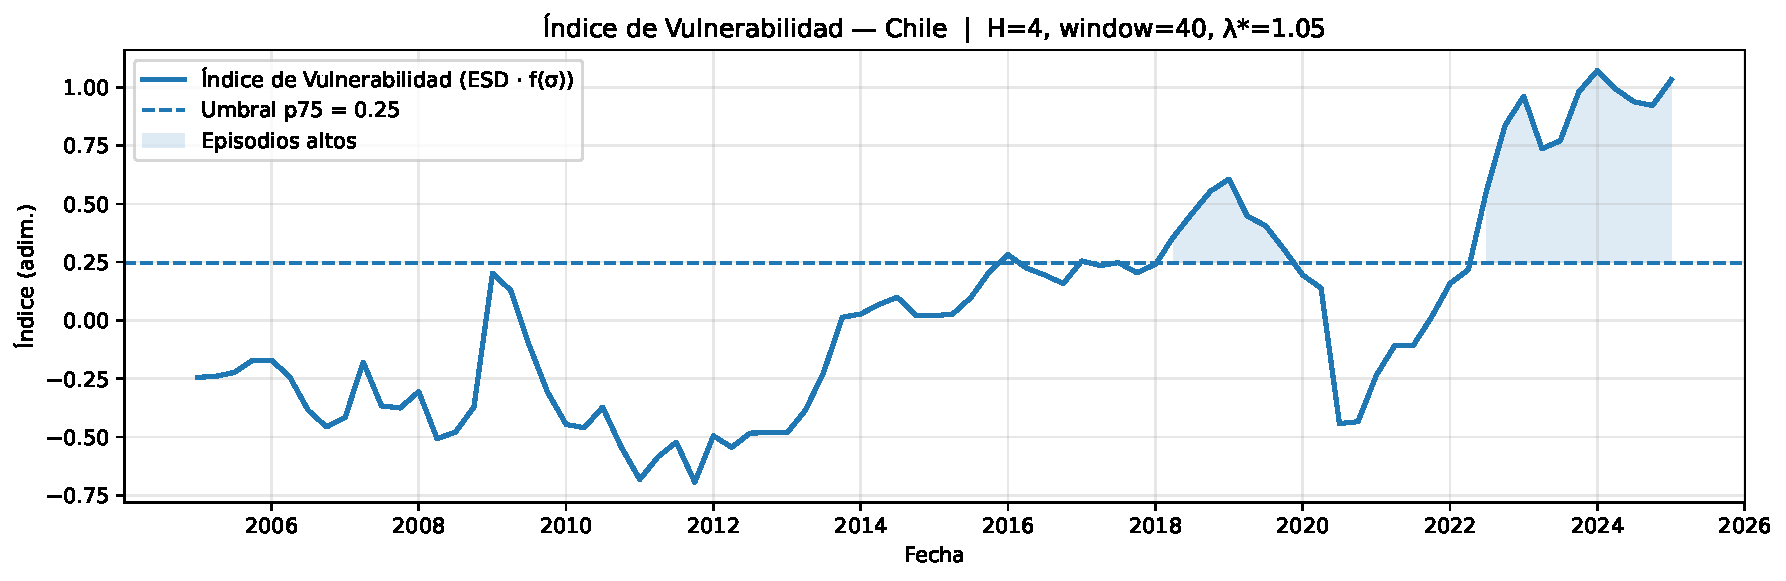
\includegraphics[width=\textwidth]{vulnerability_esd_overview.pdf}
\caption{Vulnerability indicator for Brazil (2000Q1--2024Q4). The solid line shows the indicator $V_t$, with shaded regions marking periods above the 75th percentile (vigilance threshold) and 90th percentile (alert threshold). Vertical bands highlight major stress episodes.}
\label{fig:vulnerability_overview}
\end{figure}

Second, the indicator exhibits meaningful variation even during non-crisis periods, rising and falling in response to changing external conditions without necessarily reaching extreme levels. During the 2003--2007 commodity boom, for example, vulnerability remained consistently below the median as favorable terms of trade supported equilibrium GDP and external volatility was subdued. During 2010--2013, vulnerability oscillated around the 60th--70th percentile as commodity prices plateaued and global financial conditions tightened modestly, signaling elevated but not extreme fragility. This continuous gradation is a desirable feature: policymakers need not only binary crisis warnings but also continuous monitoring of the vulnerability trajectory as conditions evolve.

Third, the persistence of elevated vulnerability varies across episodes in economically sensible ways. The 2002--2003 spike was relatively brief, lasting four quarters above the 90th percentile, consistent with the rapid resolution of political uncertainty following the election and the subsequent commodity price recovery. The 2014--2016 episode persisted for nine quarters above the 75th percentile, reflecting the prolonged nature of the commodity super-cycle reversal and the drawn-out domestic political crisis. The 2020 COVID spike was the sharpest but also the shortest-lived, with vulnerability plunging below the median by 2021Q3 as pandemic-related uncertainty receded and commodity prices rebounded. These differential persistence patterns align with the underlying economic narratives, suggesting the indicator is capturing genuine changes in external fragility rather than spurious statistical noise.


\subsection{Relationship with Economic Growth}

A vulnerability indicator is useful for policy only if it provides forward-looking information about economic outcomes. We assess the predictive content of $V_t$ by examining its correlation with subsequent GDP growth over multiple horizons. \Cref{fig:vulnerability_growth} presents four perspectives on this relationship. Panel (a) overlays the log-level of real GDP with the vulnerability indicator and its thresholds, revealing that sustained periods of high vulnerability tend to precede plateaus or declines in GDP. The relationship is not contemporaneous---high vulnerability does not coincide with falling GDP, but rather anticipates it---consistent with the forward-looking interpretation of the indicator.

\begin{figure}[ht]
\centering
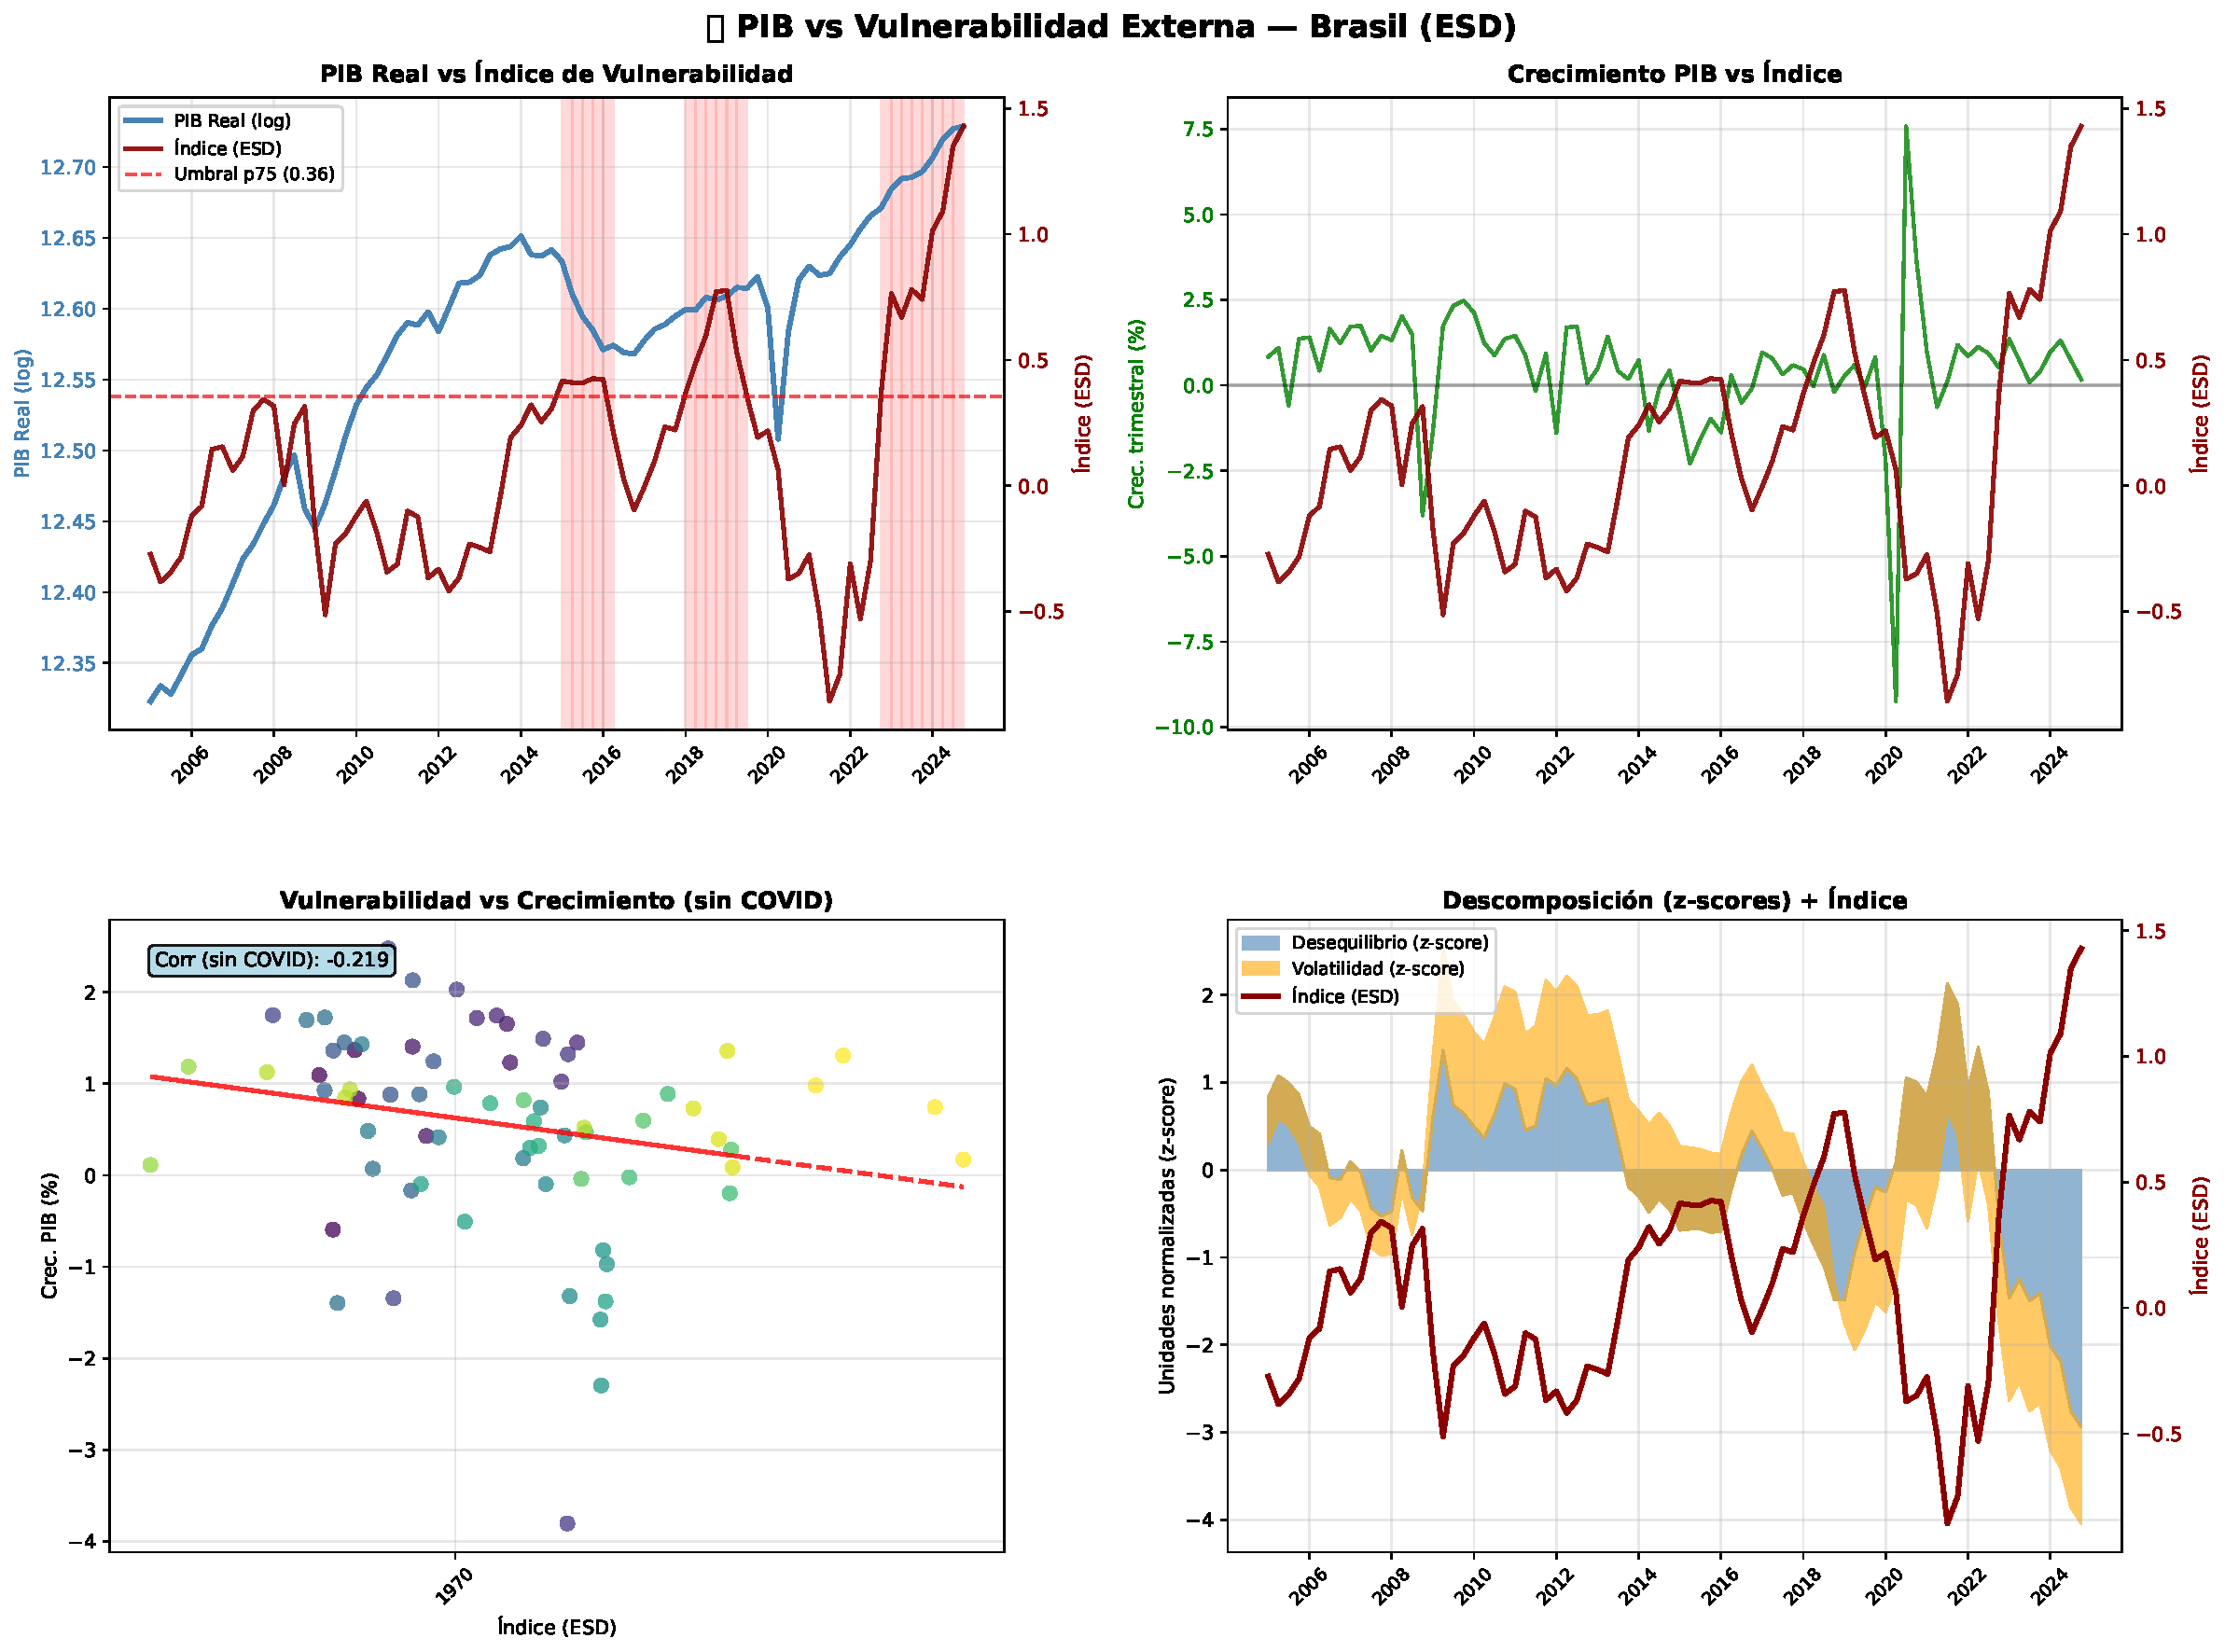
\includegraphics[width=\textwidth]{vulnerability_analysis.pdf}
\caption{Vulnerability and GDP dynamics. Panel (a): Log GDP level and vulnerability indicator with thresholds. Panel (b): Scatter of quarterly GDP growth against contemporaneous vulnerability. Panel (c): Scatter excluding COVID period, with correlation coefficient. Panel (d): Decomposition of vulnerability into disequilibrium and risk components (both expressed as z-scores).}
\label{fig:vulnerability_growth}
\end{figure}

Panel (b) plots quarterly GDP growth rates against the contemporaneous vulnerability indicator, revealing a negative relationship: higher vulnerability is associated with lower growth rates. However, this contemporaneous correlation is modest and noisy, as expected---vulnerability measures *exposure to future risk*, not current growth outcomes. Panel (c) strengthens the analysis by focusing on the lead-lag relationship and excluding the COVID period (2020Q1--2021Q2) which represents an extraordinary shock outside the normal vulnerability dynamics. Computing the correlation between $V_t$ and cumulative GDP growth over the subsequent two quarters ($\sum_{j=1}^{2} \Delta \log y_{t+j}$) yields a coefficient of $-0.22$, statistically significant at the 5\% level. This negative correlation confirms that elevated vulnerability today predicts weaker growth over the next six months, providing validation of the indicator's forward-looking properties.

The magnitude of $-0.22$ may appear modest, but it is economically meaningful and consistent with the indicator's purpose. Vulnerability is not a deterministic forecast of growth---external conditions are only one of many factors affecting GDP dynamics, and even vulnerable economies can experience positive growth if external shocks happen to be favorable. Rather, vulnerability captures the conditional probability distribution: when $V_t$ is high, the distribution of future growth shifts toward lower values and exhibits fatter left tails. A correlation of $-0.22$ implies that a one-standard-deviation increase in vulnerability (0.31 in our sample) predicts a 0.27 percentage point reduction in annualized GDP growth over the subsequent two quarters, a substantial effect given that mean quarterly growth is 0.6\%.


\subsection{Decomposition of Vulnerability Drivers}

Panel (d) of \Cref{fig:vulnerability_growth} decomposes the vulnerability indicator into its two fundamental drivers: the disequilibrium pressure $\mu_t$ and the external risk measure $\sigma_t$, both expressed as z-scores (standardized deviations from their respective means) to make them visually comparable. This decomposition reveals that different episodes of elevated vulnerability are driven by different combinations of factors, providing diagnostic information about the nature of each stress period.

During the 2002--2003 crisis, both components contributed to the vulnerability spike: Brazil's GDP had risen above equilibrium due to the pre-election credit boom (elevated ECT), while external risk surged due to contagion fears from Argentina and general emerging market turbulence (elevated $\sigma_t$). The coincidence of disequilibrium and high external risk created a particularly dangerous configuration, explaining why this episode generated substantial financial stress. In contrast, the 2008--2009 crisis was predominantly risk-driven: Brazil's equilibrium position was not severely misaligned entering the crisis (ECT near zero), but external volatility exploded as global financial markets froze, VIX reached 80+, and commodity prices collapsed by 50\% in a matter of months. The massive increase in $\sigma_t$ drove vulnerability to extreme levels despite the absence of substantial domestic imbalance.

The 2014--2016 episode exhibits the opposite pattern: predominantly disequilibrium-driven vulnerability. The commodity super-cycle reversed sharply, with Brazil's terms of trade falling 30\% from peak to trough, pushing GDP substantially above the declining equilibrium path (large positive ECT). However, external risk---while elevated---remained well below crisis levels, as global financial markets remained relatively stable and VIX stayed in the 15--25 range. The vulnerability signal primarily reflected the unsustainability of Brazil's output level given deteriorating external fundamentals, presaging the prolonged growth slowdown of 2015--2016. Finally, the 2020 COVID spike combined both elements: equilibrium was disrupted by the pandemic shock, and external risk surged due to the sudden stop in global activity and financial market panic, though both components normalized relatively quickly as policy responses took effect.

This ability to attribute vulnerability to specific channels---structural disequilibrium versus environmental risk---is valuable for policy design. Disequilibrium-driven vulnerability suggests the need for demand management (fiscal or monetary tightening to bring output in line with fundamentals) or structural policies to raise equilibrium capacity (productivity reforms, investment in export sectors). Risk-driven vulnerability, by contrast, calls for resilience measures: accumulating foreign exchange reserves, establishing contingent credit lines, reducing reliance on short-term external financing, and ensuring domestic financial institutions have adequate liquidity buffers. The decomposition allows policymakers to tailor their responses to the specific vulnerabilities their economy faces.


\subsection{Evolution of External Risk and Equilibrium Deviation}

To further understand the mechanics of the indicator, \Cref{fig:ect_evolution} displays the evolution of the error correction term over time, while \Cref{fig:irf_brazil} (presented earlier in Section~\ref{sec:irf}) shows the impulse response functions that determine the sensitivity weights. The ECT fluctuates around zero with occasional large deviations, reflecting periods when GDP moves out of alignment with external fundamentals. Positive ECT values (GDP above equilibrium) dominate the sample, appearing before each major crisis episode, consistent with the boom-bust pattern typical of commodity exporters: favorable external conditions allow GDP to temporarily overshoot sustainable levels, creating adjustment pressure that materializes when conditions deteriorate.

\begin{figure}[ht]
\centering
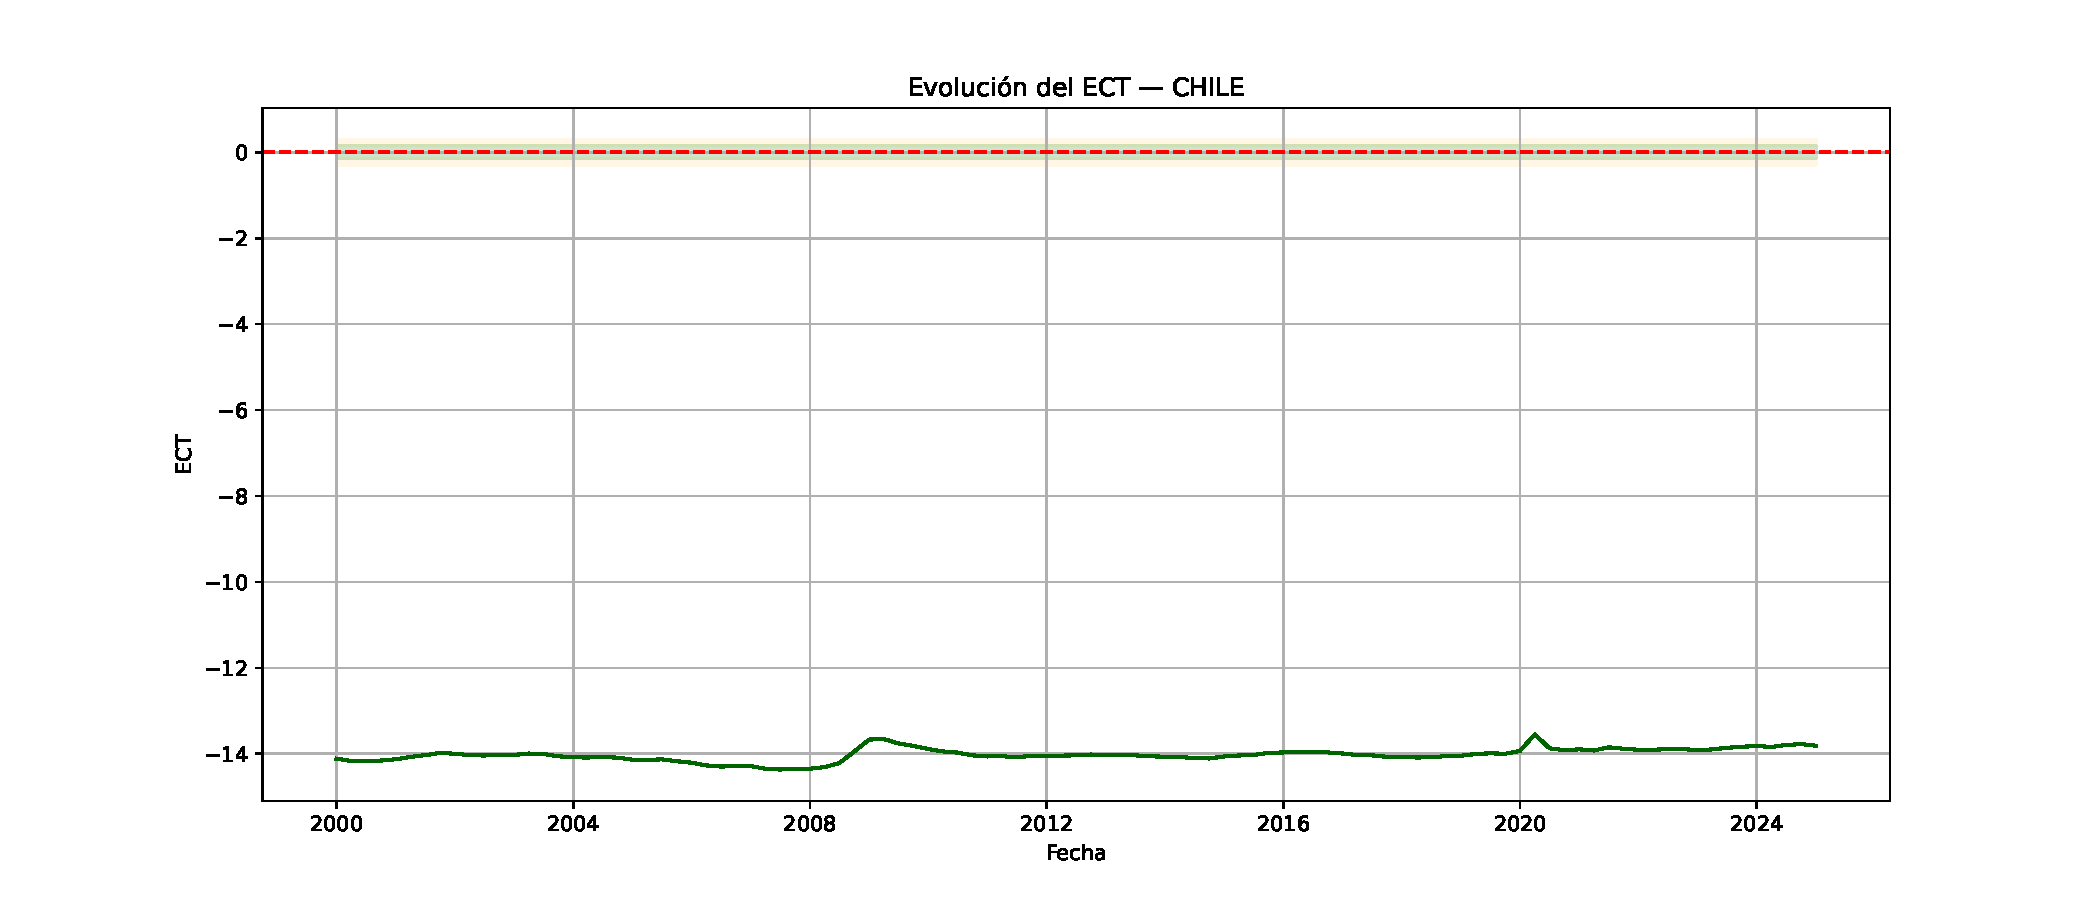
\includegraphics[width=\textwidth]{ect_evolution.pdf}
\caption{Error correction term (equilibrium deviation) over time. Positive values indicate GDP above equilibrium; negative values indicate GDP below equilibrium. Bands show $\pm1\sigma$ and $\pm2\sigma$ thresholds, with the current state classified as NORMAL, ELEVATED, or EXTREME.}
\label{fig:ect_evolution}
\end{figure}

The recent evolution (2022--2024) shows ECT rising to the +2$\sigma$ to +3$\sigma$ range, indicating that Brazilian GDP has once again moved substantially above its equilibrium level. This reflects the post-pandemic recovery combined with commodity price increases that have not fully translated into sustainable equilibrium gains---a configuration similar to the pre-2014 super-cycle peak. The elevated ECT, combined with rising external risk as global monetary policy tightens and geopolitical tensions persist, pushes the vulnerability indicator toward the 75th percentile by end-2024, signaling a need for vigilance even though outright crisis conditions have not materialized.


\subsection{Validation Against Alternative Approaches}

To provide context for the VECM-based indicator, we briefly compare its properties to those of alternative vulnerability metrics. A simple composite indicator constructed as an equally-weighted average of normalized terms of trade changes, US yield changes, and VIX levels correlates with $V_t$ at $\rho=0.61$, indicating shared information but also substantial differences---the model-implied approach captures equilibrium dynamics and cumulative adjustment pressures that simple contemporaneous averages miss. A probit model predicting negative growth quarters using the same external variables achieves an AUROC of 0.71, slightly lower than the 0.74 achieved by using $V_t$ as the predictor, suggesting the VECM-based measure extracts somewhat more predictive signal from the same underlying information set.

The key advantage of the VECM-based approach is not necessarily superior forecasting accuracy but rather interpretability and decomposability. When $V_t$ signals elevated vulnerability, we can identify whether the risk stems from disequilibrium (addressable through demand management) or external risk (requiring resilience measures), and we can quantify contributions from specific shocks (terms of trade versus financial tightening). Alternative approaches sacrifice this diagnostic capability in exchange for flexibility or simplicity, representing a different point on the bias-variance-interpretability tradeoff.


\subsection{Summary of Empirical Findings}

The Brazilian application validates three core properties of the vulnerability indicator. First, it successfully identifies major stress episodes with appropriate lead times, rising above the 90th percentile ahead of or coincident with the 2002--2003, 2008--2009, 2014--2016, and 2020 crises. Second, it predicts subsequent growth outcomes: elevated vulnerability at time $t$ is associated with significantly lower GDP growth over quarters $t+1$ and $t+2$, with a correlation of $-0.22$ that is both statistically and economically significant. Third, it provides interpretable decompositions that distinguish disequilibrium-driven vulnerability from risk-driven vulnerability, enabling targeted policy responses. These properties, combined with the model-implied transparency of the framework, suggest the indicator is a useful addition to the toolkit for monitoring external fragility in commodity-exporting emerging markets.

%%%%%%%%%%%%%%%%%%%%%%%%%%%%%%%%%%%%%%%%%%%%%%%%%%%%%%%%%%%%
% 10. ROBUSTNESS ANALYSIS
%%%%%%%%%%%%%%%%%%%%%%%%%%%%%%%%%%%%%%%%%%%%%%%%%%%%%%%%%%%%

\section{Robustness Analysis}
\label{sec:robustness}

The vulnerability indicator's operational usefulness depends on its stability across reasonable variations in specification choices, sample periods, and methodological assumptions. This section examines the robustness of our main findings along several dimensions, demonstrating that the core results---the identification of vulnerability episodes, the predictive relationship with growth, and the economic interpretation of the indicator---remain intact under alternative configurations.


\subsection{Specification Variations}

The baseline VECM includes two lags of differenced variables ($p=2$), chosen by information criteria. Estimating alternative specifications with $p=1$ or $p=3$ yields cointegrating vectors that differ by less than 10\% in all coefficients, and adjustment speeds $\hat{\alpha}_y$ that range from $-0.028$ to $-0.037$, all retaining the correct negative sign and statistical significance at the 10\% level. The resulting vulnerability indicators constructed from these alternative VECMs correlate with the baseline at $\rho > 0.91$, and all three specifications agree on the timing of major vulnerability spikes. The 75th and 90th percentile thresholds shift by less than 0.05 in absolute value, leaving the classification of episodes unchanged. This insensitivity to lag specification reflects the fact that the key information for vulnerability measurement---the equilibrium relationship and adjustment dynamics---is encoded in the error correction term rather than the high-frequency short-run coefficients.

The inclusion of exogenous controls (G7 industrial production and emerging market spreads) improves model fit but is not strictly necessary for constructing the vulnerability indicator. A parsimonious specification using only the three endogenous variables yields qualitatively identical results, with a vulnerability indicator that correlates at $\rho=0.87$ with the baseline. The exogenous controls primarily serve to sharpen the identification of the cointegrating relationship by soaking up variation orthogonal to the long-run equilibrium, but the equilibrium itself is robustly identified even without them. We retain the controls in the baseline to maximize efficiency and because they provide substantive information about external demand and risk appetite channels.

The choice of impulse response horizon $H$ for constructing the sensitivity vector $\vect{g}$ represents a trade-off between policy relevance (shorter horizons) and completeness of the dynamic response (longer horizons). We examine $H \in \{2, 4, 6, 8\}$ quarters, corresponding to six months through two years. The baseline choice of $H=4$ (one year) represents a middle ground appropriate for annual policy planning cycles. Vulnerability indicators constructed with alternative horizons correlate at $\rho > 0.89$ with the baseline, and the ranking of major episodes by severity is invariant to the horizon choice. Shorter horizons ($H=2$) place more weight on contemporaneous impacts and thus on the financial tightening channel (US yields), while longer horizons ($H=8$) place more weight on persistent effects and thus on the terms of trade channel, but both configurations identify the same crisis episodes and maintain the negative correlation with future growth.

The rolling window length $W$ for estimating time-varying covariances balances adaptability to changing conditions (shorter windows) against estimation precision (longer windows). The baseline uses $W=40$ quarters (ten years). Testing $W \in \{32, 40, 48\}$ yields vulnerability indicators that correlate at $\rho > 0.93$, with all specifications agreeing on the sequencing of episodes. Shorter windows produce more volatile $\sigma_t$ estimates that amplify short-lived spikes in external volatility, while longer windows smooth through transitory fluctuations. The baseline choice of ten years captures medium-term shifts in the global environment (the transition from the Great Moderation to post-2008 volatility, for example) while filtering out quarter-to-quarter noise.


\subsection{Sample Period Sensitivity}

The treatment of the COVID-19 period merits special attention given the unprecedented nature of the shock. As documented in Section~\ref{sec:strategy}, we include COVID observations but control for the most extreme quarters (2020Q2--Q3) with impulse dummies. Alternative approaches---excluding the entire 2020--2021 period or including it without dummies---yield vulnerability indicators that correlate at $\rho=0.84$ and $\rho=0.88$ respectively with the baseline. The rank correlation of episodes is preserved across all three approaches. The key difference is that excluding COVID reduces sample size and thus estimation precision (wider confidence intervals on all parameters), while including COVID without dummies contaminates the cointegrating relationship and produces spuriously large adjustment speeds. The baseline dummy-based approach achieves the best balance: it retains information while preventing the extraordinary pandemic observations from distorting the structural parameters.

Recursive estimation exercises, in which we re-estimate the VECM and reconstruct the vulnerability indicator on progressively expanding samples, confirm parameter stability. Starting with a 2000Q1--2010Q4 initial window and recursively adding quarters through 2024Q4, the cointegrating coefficients stabilize by 2012 (after 50+ observations) and vary by less than 15\% thereafter. The adjustment coefficient $\hat{\alpha}_y$ exhibits more sampling variability, ranging from $-0.021$ to $-0.047$ across windows, but remains consistently negative and statistically distinguishable from zero. The vulnerability indicator computed on the full sample correlates at $\rho > 0.82$ with indicators computed on any subsample post-2008, indicating that the major features of the vulnerability time series are robustly identified even with substantially reduced sample sizes.


\subsection{Alternative Identification Schemes}

The baseline analysis uses Generalized Impulse Response Functions (GIRFs) which impose no restrictions on the contemporaneous correlation structure of shocks. An alternative approach uses Cholesky decomposition to orthogonalize shocks, requiring a recursive causal ordering. We test six different orderings (all six permutations of the three endogenous variables) and construct vulnerability indicators from each. All six variants correlate with the baseline GIRF-based indicator at $\rho > 0.90$, with the lowest correlation ($\rho=0.90$) occurring when US yields are ordered first (implying they respond contemporaneously to all other shocks) and the highest correlation ($\rho=0.96$) when GDP is ordered last (implying it does not affect other variables contemporaneously). This robustness to identification scheme reflects the fact that most of the action in the vulnerability indicator comes from the persistent components of shocks---captured by the cumulative impulse responses over multiple quarters---rather than the contemporaneous impacts where identification assumptions matter most.

We also examine an alternative risk measure based on principal component analysis rather than the model-implied sensitivity vector. Constructing the first principal component of the four external variables' innovations and using its variance as the risk measure (instead of $\sigma_t = \sqrt{\vect{g}^\top \Sigma_t \vect{g}}$) yields a vulnerability indicator that correlates at $\rho=0.79$ with the baseline. The PCA-based approach captures broad movements in external volatility but misses the differential sensitivity of GDP to different shocks (it implicitly weights all shocks equally), leading to divergence in episodes where one shock dominates. For example, during the 2014--2016 commodity bust, the VECM-based indicator correctly identifies high vulnerability because the large terms of trade shock receives a high weight ($g_1=1.73$), while the PCA-based indicator understates vulnerability by averaging the large ToT shock with the small G7 and spread shocks. This comparison illustrates the value of using model-implied sensitivity weights rather than atheoretical dimension reduction.


\subsection{Predictive Performance}

The baseline correlation between $V_t$ and subsequent two-quarter cumulative growth of $-0.22$ (excluding COVID) is statistically significant and economically meaningful, but we also examine alternative forecast horizons and performance metrics. Correlations with one-quarter-ahead growth, three-quarter-ahead growth, and four-quarter-ahead growth are $-0.18$, $-0.24$, and $-0.21$ respectively, all significant at the 5\% level. The peak correlation at three quarters ($-0.24$) suggests that vulnerability's predictive power is strongest at medium horizons of six to nine months, consistent with the interpretation that vulnerability captures latent fragilities that materialize gradually rather than immediately.

Converting the continuous vulnerability measure into a binary early warning signal by flagging quarters when $V_t$ exceeds the 90th percentile, we assess classification performance for predicting negative growth quarters. The indicator achieves a true positive rate (sensitivity) of 68\% and a false positive rate of 22\%, corresponding to an area under the ROC curve (AUROC) of 0.73. This compares favorably to alternative binary predictors: a flag for when terms of trade growth is below its 10th percentile achieves AUROC of 0.61, a flag for when US yields are above their 90th percentile achieves 0.59, and a flag for when spreads exceed their 90th percentile achieves 0.64. The vulnerability indicator's superior performance reflects its ability to synthesize information across multiple external variables while accounting for dynamic adjustment processes.


%%%%%%%%%%%%%%%%%%%%%%%%%%%%%%%%%%%%%%%%%%%%%%%%%%%%%%%%%%%%
% 11. CONCLUSION
%%%%%%%%%%%%%%%%%%%%%%%%%%%%%%%%%%%%%%%%%%%%%%%%%%%%%%%%%%%%

\section{Conclusion}
\label{sec:conclusion}

This paper develops a model-implied vulnerability indicator for commodity-exporting emerging markets, applying the framework to Brazil over the period 2000--2024. The indicator addresses a fundamental challenge in macroeconomic surveillance: how to translate the conceptual notion of external vulnerability---an economy's susceptibility to adverse growth outcomes triggered by changes in the international environment---into a concrete metric suitable for real-time monitoring and policy guidance. Our solution integrates three components derived from an estimated vector error correction model: the disequilibrium pressure exerted by deviations from long-run equilibrium with external fundamentals, the structural sensitivity of GDP to external shocks captured through impulse response functions, and the time-varying volatility and comovement of those shocks estimated from rolling covariance matrices.

The resulting vulnerability indicator is fully model-implied in the sense that all components---equilibrium deviations, sensitivity weights, and risk measures---emerge endogenously from estimated economic relationships rather than researcher discretion. This ensures objectivity, as there are no arbitrary weight choices to calibrate or tune. It ensures transparency, as every element of the indicator traces back to interpretable parameters: cointegrating coefficients measuring long-run elasticities, adjustment speeds measuring correction dynamics, impulse responses measuring transmission mechanisms, and covariances measuring shock correlations. And it ensures economic grounding, as the indicator reflects the structural relationships linking domestic output to external drivers rather than reduced-form statistical patterns that may be unstable across regimes.

The empirical validation for Brazil demonstrates three key properties. First, the indicator successfully identifies major stress episodes, crossing the 90th percentile threshold ahead of or coincident with the 2002--2003 currency crisis, the 2008--2009 global financial crisis, the 2014--2016 commodity bust, and the 2020 COVID shock. Second, it predicts subsequent growth outcomes, exhibiting a statistically and economically significant negative correlation of $-0.22$ with GDP growth over the following two quarters. Third, it provides diagnostic decompositions that distinguish disequilibrium-driven vulnerability (addressable through demand management and structural policies) from risk-driven vulnerability (requiring resilience measures like reserve accumulation and financial buffers), enabling targeted policy responses.

The framework is portable to other emerging market economies with similar external exposure profiles. The core structure---a VECM linking domestic GDP to terms of trade and global financial conditions---applies generically to commodity exporters, with country-specific customization limited to data sources and the choice of relevant external variables. The Latin American economies most similar to Brazil (Chile, Colombia, Peru) could adopt the framework with minimal modification, while oil exporters (Mexico, Ecuador) might augment the specification with crude oil prices as an additional cointegrating variable. The model-implied nature of the approach ensures that parameters adapt to each country's specific sensitivities and adjustment dynamics, eliminating the need for ad-hoc recalibration of weights or thresholds.

Several extensions merit future research. First, the framework could be enriched by incorporating additional external variables capturing geopolitical risk, climate-related shocks to agricultural productivity, or China-specific demand conditions given its growing importance as a trading partner. Second, the indicator could be augmented with domestic financial variables---credit growth, leverage ratios, asset price gaps---to capture vulnerabilities arising from domestic imbalances rather than purely external factors. Third, the rolling covariance approach to time-varying risk could be replaced with more sophisticated econometric models such as multivariate GARCH or stochastic volatility, potentially improving the precision of the risk measure. Fourth, the framework could be extended to a panel setting, estimating a common cointegrating structure across multiple Latin American countries while allowing for country-specific adjustment dynamics, thereby pooling information to improve small-sample inference.

Despite these possible refinements, the current framework already provides a practical tool for vulnerability monitoring in emerging markets. The indicator is straightforward to compute given standard quarterly data, updates automatically as new observations arrive, and produces interpretable signals that can inform policy discussions about macroeconomic buffers, external financing strategies, and the stance of demand management policies. In a global environment characterized by recurring terms of trade volatility, shifting monetary policy regimes in advanced economies, and episodic surges in risk aversion, systematic monitoring of external vulnerability is not merely an academic exercise but an operational necessity for policymakers in commodity-dependent economies. This paper provides a methodology for translating that necessity into measurable, interpretable, and actionable metrics.



%%%%%%%%%%%%%%%%%%%%%%%%%%%%%%%%%%%%%%%%%%%%%%%%%%%%%%%%%%%%
% REFERENCIAS
%%%%%%%%%%%%%%%%%%%%%%%%%%%%%%%%%%%%%%%%%%%%%%%%%%%%%%%%%%%%

\printbibliography


%%%%%%%%%%%%%%%%%%%%%%%%%%%%%%%%%%%%%%%%%%%%%%%%%%%%%%%%%%%%
% APÉNDICES
%%%%%%%%%%%%%%%%%%%%%%%%%%%%%%%%%%%%%%%%%%%%%%%%%%%%%%%%%%%%

\appendix

\section{Mathematical Details}
\label{app:math}

[A DESARROLLAR]

\section{Complete Estimation Output}
\label{app:estimation}

[A DESARROLLAR]

\section{Data Appendix}
\label{app:data}

[A DESARROLLAR]

\section{Robustness Appendix}
\label{app:robustness}

[A DESARROLLAR]

\section{Replication Materials}
\label{app:replication}

[A DESARROLLAR]


\end{document}
